\documentclass{amsart}
% !TEX root = ../cobar1.tex

\usepackage{microtype}
\usepackage{amssymb}
\usepackage{mathtools}
\usepackage{tikz-cd}
\usepackage{mathbbol} % changes \mathbb{} and adds more support

% bibliography
\usepackage[
	backend=biber,
	style=alphabetic,
	backref=true,
	url=false,
	doi=false,
	isbn=false,
	eprint=false]{biblatex}

\renewbibmacro{in:}{}  % don't display "in:" before the journal name
\AtEveryBibitem{\clearfield{pages}}  % don't show page numbers

\DeclareFieldFormat{title}{\myhref{\mkbibemph{#1}}}
\DeclareFieldFormat
[article,inbook,incollection,inproceedings,patent,thesis,unpublished]
{title}{\myhref{\mkbibquote{#1\isdot}}}

\newcommand{\doiorurl}{%
	\iffieldundef{url}
	{\iffieldundef{eprint}
		{}
		{http://arxiv.org/abs/\strfield{eprint}}}
	{\strfield{url}}%
}

\newcommand{\myhref}[1]{%
	\ifboolexpr{%
		test {\ifhyperref}
		and
		not test {\iftoggle{bbx:eprint}}
		and
		not test {\iftoggle{bbx:url}}
	}
	{\href{\doiorurl}{#1}}
	{#1}%
}

% references
\usepackage[
	bookmarks=true,
	linktocpage=true,
	bookmarksnumbered=true,
	breaklinks=true,
	pdfstartview=FitH,
	hyperfigures=false,
	plainpages=false,
	naturalnames=true,
	colorlinks=true,
	pagebackref=false,
	pdfpagelabels]{hyperref}

\hypersetup{
	colorlinks,
	citecolor=blue,
	filecolor=blue,
	linkcolor=blue,
	urlcolor=blue
}

\usepackage[capitalize, noabbrev]{cleveref}
\let\subsectionSymbol\S
\crefname{subsection}{\subsectionSymbol\!\!}{subsections}

% layout
\addtolength{\textwidth}{0in}
\addtolength{\textheight}{0in}
\calclayout

% update to MSC2020
\makeatletter
\@namedef{subjclassname@2020}{%
	\textup{2020} Mathematics Subject Classification}
\makeatother

% table of contents
\setcounter{tocdepth}{4}

% !TEX root = ../cobar1.tex

\newcommand{\s}[1]{s^{\scalebox{.6}{{#1}}}}
\DeclareMathOperator{\aug}{\varepsilon}

\newcommand{\Smod}{\mathsf{Mod}_{\S}}
\newcommand{\Sbimod}{\mathsf{biMod}_{\S}}
\newcommand{\graphs}{\mathfrak{G}}
\renewcommand{\S}{\mathbb{S}}
\newcommand{\biEnd}{\mathrm{biEnd}}

\newcommand{\As}{{\mathcal{A}\mathsf{s}}}
\newcommand{\Com}{\cC{om}}
\newcommand{\M}{\cM}
\newcommand{\UM}{{\forget(\M)}}
\newcommand{\USL}{{\forget(\M_{sl})}}

\DeclareMathOperator{\adams}{A}
\DeclareMathOperator{\adamsE}{\widehat{A}}
\DeclareMathOperator{\adamsEA}{\widehat{A}_{\!\As}}
\DeclareMathOperator{\adamsEUM}{\widehat{A}_{\UM}}

\DeclareMathOperator{\schains}{N^{\simplex}}
\DeclareMathOperator{\cchains}{N^{\cube}}
\DeclareMathOperator{\scochains}{N^{\vee}_{\simplex}}
\DeclareMathOperator{\ccochains}{N^{\vee}_{\cube}}
\DeclareMathOperator{\Schains}{S}
\DeclareMathOperator{\sSchains}{S^{\simplex}}
\DeclareMathOperator{\cSchains}{S^{\cube}}
\DeclareMathOperator{\schainsA}{N^{\simplex}_{\!\As}}
\DeclareMathOperator{\cchainsA}{N^{\cube}_{\!\As}}
\DeclareMathOperator{\SchainsA}{S_{\!\As}}
\DeclareMathOperator{\sSchainsA}{S^{\simplex}_{\!\As}}
\DeclareMathOperator{\cSchainsA}{S^{\cube}_{\!\As}}
\DeclareMathOperator{\sSchainsUM}{S^{\simplex}_{\UM}}
\DeclareMathOperator{\cSchainsUM}{S^{\cube}_{\UM}}
\DeclareMathOperator{\schainsUM}{N^{\simplex}_{\UM}}
\DeclareMathOperator{\cchainsUM}{N^{\cube}_{\UM}}
\DeclareMathOperator{\schainsUSL}{N^{\simplex}_{\USL}}
\DeclareMathOperator{\cchainsUSL}{N^{\cube}_{\USL}}

\DeclareMathOperator{\sSing}{Sing^{\simplex}}
\DeclareMathOperator{\cSing}{Sing^{\cube}}

\DeclareMathOperator{\ccobar}{\mathbb{\Omega}}
\DeclareMathOperator{\ccobarE}{\widehat{\mathbb{\Omega}}}
\DeclareMathOperator{\ncobar}{\mathbb{\Omega}^{\mathrm{nec}}}
\DeclareMathOperator{\ncobarE}{\widehat{\mathbb{\Omega}}^{\mathrm{nec}}}

\DeclareMathOperator{\cartanserre}{\xi}
\DeclareMathOperator{\rigid}{\mathfrak{C}}
\DeclareMathOperator{\nerve}{\mathfrak{N}}
\DeclareMathOperator{\classifying}{\overline{W}}
\DeclareMathOperator{\localization}{\mathcal{L}}
\DeclareMathOperator{\kan}{G}
\DeclareMathOperator{\triangulate}{\mathcal{T}}

\newcommand{\Nec}{\mathsf{Nec}}
\newcommand{\nSet}{\mathsf{nSet}}

\newcommand{\manuel}[1]{\textcolor{red}{\underline{Manuel}: #1}}

\newcommand{\pdfM}{\texorpdfstring{${\cM}$}{M}}

\title[The cobar construction as an $E_{\infty}$-bialgebra]{The cobar construction as an $E_{\infty}$-bialgebra model of the based loop space}

\author[A. Medina-Mardones]{Anibal M. Medina-Mardones}
\address{A.M-M., Max Plank Institute for Mathematics \and University of Notre Dame}
\email{\href{mailto:ammedmar@mpim-bonn.mpg.de}{ammedmar@mpim-bonn.mpg.de}}

\author[M. Rivera]{Manuel Rivera}
\address{M.R., Department of Mathematics, Purdue University}
\email{\href{mailto:manuelr@purdue.edu}{manuelr@purdue.edu}}

\subjclass[2020]{57T30, 55P35, 18N70, 55U10, 55N45, 55S05}
\keywords{cobar construction, ${E_\infty}$-structures, loop spaces, simplicial sets, Steenrod operations}

\usetikzlibrary{arrows,decorations.markings}
\tikzset{myptr/.style={decoration={markings,mark=at position 1 with %
			{\arrow[scale=2,>=stealth]{>}}},postaction={decorate}}}
		
\newsavebox\preproduct
\begin{lrbox}{\preproduct}
	\begin{tikzpicture}[scale=.3]
	\draw (0,0)--(0,-.8);
	\draw (0,0)--(.5,.5);
	\draw (0,0)--(-.5,.5);
	\end{tikzpicture} 
\end{lrbox}
\newcommand{\product}{% <- this 'right of' is inherited; how to avoid?
	\usebox\preproduct}

\newsavebox\precoproduct
	\begin{lrbox}{\precoproduct}
		\begin{tikzpicture}[scale=.3]
		\draw (0,0)--(0,.8);
		\draw (0,0)--(.5,-.5);
		\draw (0,0)--(-.5,-.5);
		\end{tikzpicture}
	\end{lrbox}
\newcommand{\coproduct}{% <- this 'right of' is inherited; how to avoid?
	\usebox\precoproduct}

\newsavebox\preboundary
\begin{lrbox}{\preboundary}
	\begin{tikzpicture}[scale=.3]
	\draw (0,0)--(0,1.3);
	\draw (.5,0)--(.5,1.3);
	\draw [fill] (0,0) circle [radius=0.1];
	\draw (.9,.6)--(1.3,.6);
	\draw (1.7,0)--(1.7,1.3);
	\draw (2.2,0)--(2.2,1.3);
	\draw [fill] (2.2,0) circle [radius=0.1];
	\end{tikzpicture}
\end{lrbox}
\newcommand{\boundary}{% <- this 'right of' is inherited; how to avoid?
	\usebox\preboundary}

\newsavebox\preleftboundary
\begin{lrbox}{\preleftboundary}
	\begin{tikzpicture}[scale=.3]
	\draw (1.7,0)--(1.7,1.3);
	\draw (2.2,0)--(2.2,1.3);
	\draw [fill] (2.2,0) circle [radius=0.1];
	\end{tikzpicture}
\end{lrbox}
\newcommand{\leftboundary}{% <- this 'right of' is inherited; how to avoid?
	\usebox\preleftboundary}

\newsavebox\prerightboundary
\begin{lrbox}{\prerightboundary}
	\begin{tikzpicture}[scale=.3]
	\draw (0,0)--(0,1.3);
	\draw (.5,0)--(.5,1.3);
	\draw [fill] (0,0) circle [radius=0.1];
	\end{tikzpicture}
\end{lrbox}
\newcommand{\rightboundary}{% <- this 'right of' is inherited; how to avoid?
	\usebox\prerightboundary}

\newsavebox\precoboundary
\begin{lrbox}{\precoboundary}
	\begin{tikzpicture}[scale=.3]
	\draw (0,0)--(0,1.3);
	\draw (.5,0)--(.5,1.3);
	\draw [fill] (0,1.3) circle [radius=0.1];
	\draw (.9,.6)--(1.3,.6);
	\draw (1.7,0)--(1.7,1.3);
	\draw (2.2,0)--(2.2,1.3);
	\draw [fill] (2.2,1.3) circle [radius=0.1];
	\end{tikzpicture}
\end{lrbox}
\newcommand{\coboundary}{% <- this 'right of' is inherited; how to avoid?
	\usebox\precoboundary}

\newsavebox\precounit
\begin{lrbox}{\precounit}
	\begin{tikzpicture}[scale=.3]
	\draw (0,0)--(0,1.3);
	\draw [fill] (0,0) circle [radius=0.1];
	\end{tikzpicture}
\end{lrbox}
\newcommand{\counit}{% <- this 'right of' is inherited; how to avoid?
	\usebox\precounit}

\newsavebox\preidentity
\begin{lrbox}{\preidentity}
	\begin{tikzpicture}[scale=.3]
	\draw (0,0)--(0,1.3);
	\end{tikzpicture}
\end{lrbox}
\newcommand{\identity}{% <- this 'right of' is inherited; how to avoid?
	\usebox\preidentity}

\newsavebox\preunit
\begin{lrbox}{\preunit}
	\begin{tikzpicture}[scale=.3]
	\draw (0,0)--(0,1.3);
	\draw [fill] (0,1.3) circle [radius=0.1];
	\end{tikzpicture}
\end{lrbox}
\newcommand{\unit}{% <- this 'right of' is inherited; how to avoid?
	\usebox\preunit}

\newsavebox\preassociativity
\begin{lrbox}{\preassociativity}
	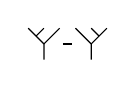
\begin{tikzpicture}[scale=.2]
	\path[draw] (0,0)--(0,1)--(-1,2);
	\draw (0,1)--(1,2);
	\draw (-.5,1.5)--(0,2);
	\draw (1.2,1)--(1.8,1);
	\path[draw] (3,0)--(3,1)--(2,2);
	\draw (3,1)--(4,2);
	\draw (3.5,1.5)--(3,2);	
	\end{tikzpicture}
\end{lrbox}
\newcommand{\associativity}{% <- this 'right of' is inherited; how to avoid?
	\usebox\preassociativity}

\newsavebox\precoassociativity
\begin{lrbox}{\precoassociativity}
	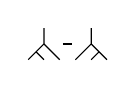
\begin{tikzpicture}[scale=.2]
	\path[draw] (0,0)--(0,-1)--(-1,-2);
	\draw (0,-1)--(1,-2);
	\draw (-.5,-1.5)--(0,-2);
	\draw (1.2,-1)--(1.8,-1);
	\path[draw] (3,0)--(3,-1)--(2,-2);
	\draw (3,-1)--(4,-2);
	\draw (3.5,-1.5)--(3,-2);
	\end{tikzpicture}
\end{lrbox}
\newcommand{\coassociativity}{% <- this 'right of' is inherited; how to avoid?
	\usebox\precoassociativity}

\newsavebox\preleftcomb
\begin{lrbox}{\preleftcomb}
	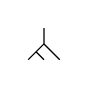
\begin{tikzpicture}[scale=.2]
	\path[draw] (0,0)--(0,-1)--(-1,-2);
	\draw (0,-1)--(1,-2);
	\draw (-.5,-1.5)--(0,-2);
	\end{tikzpicture}
\end{lrbox}
\newcommand{\leftcomb}{% <- this 'right of' is inherited; how to avoid?
	\usebox\preleftcomb}

\newsavebox\prerightcomb
\begin{lrbox}{\prerightcomb}
	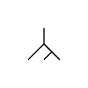
\begin{tikzpicture}[scale=.2]
	\path[draw] (3,0)--(3,-1)--(2,-2);
	\draw (3,-1)--(4,-2);
	\draw (3.5,-1.5)--(3,-2);
	\end{tikzpicture}
\end{lrbox}
\newcommand{\rightcomb}{% <- this 'right of' is inherited; how to avoid?
	\usebox\prerightcomb}

\newsavebox\preinvolution
\begin{lrbox}{\preinvolution}
	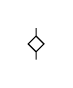
\begin{tikzpicture}[scale=.2]
	\path[draw] (0,0)--(0,.5)--(-.5,1)--(0,1.5)--(0,2);
	\path[draw] (0,.5)--(.5,1)--(0,1.5);
	\end{tikzpicture}
\end{lrbox}
\newcommand{\involution}{% <- this 'right of' is inherited; how to avoid?
	\usebox\preinvolution}

\newsavebox\preleftcounitality
\begin{lrbox}{\preleftcounitality}
	\begin{tikzpicture}[scale=.3]
	\draw (0,0)--(0,.8);
	\draw (0,0)--(.5,-.5);
	\draw (0,0)--(-.5,-.5);
	\draw [fill] (-.5,-.5) circle [radius=0.1];
	\draw (.7,0)--(1.1,0);
	\path[draw] (1.5,-.5)--(1.5,.8);
	\end{tikzpicture}
\end{lrbox}
\newcommand{\leftcounitality}{% <- this 'right of' is inherited; how to avoid?
	\usebox\preleftcounitality}

\newsavebox\preleftcounitcoproduct
\begin{lrbox}{\preleftcounitcoproduct}
	\begin{tikzpicture}[scale=.3]
	\draw (0,0)--(0,.8);
	\draw (0,0)--(.5,-.5);
	\draw (0,0)--(-.5,-.5);
	\draw [fill] (-.5,-.5) circle [radius=0.1];
	\end{tikzpicture}
\end{lrbox}
\newcommand{\leftcounitcoproduct}{% <- this 'right of' is inherited; how to avoid?
	\usebox\preleftcounitcoproduct}

\newsavebox\prerightcounitality
\begin{lrbox}{\prerightcounitality}
	\begin{tikzpicture}[scale=.3]
	\draw (0,0)--(0,.8);
	\draw (0,0)--(.5,-.5);
	\draw (0,0)--(-.5,-.5);
	\draw [fill] (.5,-.5) circle [radius=0.1];
	\draw (-.7,0)--(-1.1,0);
	\path[draw] (-1.5,-.5)--(-1.5,.8);
	\end{tikzpicture}
\end{lrbox}
\newcommand{\rightcounitality}{% <- this 'right of' is inherited; how to avoid?
	\usebox\prerightcounitality}

\newsavebox\prerightcounitcoproduct
\begin{lrbox}{\prerightcounitcoproduct}
	\begin{tikzpicture}[scale=.3]
	\draw (0,0)--(0,.8);
	\draw (0,0)--(.5,-.5);
	\draw (0,0)--(-.5,-.5);
	\draw [fill] (.5,-.5) circle [radius=0.1];
	\end{tikzpicture}
\end{lrbox}
\newcommand{\rightcounitcoproduct}{% <- this 'right of' is inherited; how to avoid?
	\usebox\prerightcounitcoproduct}

\newsavebox\preleftunitality
\begin{lrbox}{\preleftunitality}
	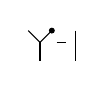
\begin{tikzpicture}[scale=.3]
	\draw (0,0)--(0,-.8);
	\draw (0,0)--(-.5,.5);
	\draw (0,0)--(.5,.5);
	\draw [fill] (.5,.5) circle [radius=0.1];
	\draw (.7,0)--(1.1,0);
	\path[draw] (1.5,.5)--(1.5,-.8);
	\end{tikzpicture}
\end{lrbox}
\newcommand{\leftunitality}{% <- this 'right of' is inherited; how to avoid?
	\usebox\preleftunitality}

\newsavebox\prerightunitality
\begin{lrbox}{\prerightunitality}
	\begin{tikzpicture}[scale=.3]
	\draw (0,0)--(0,-.8);
	\draw (0,0)--(-.5,.5);
	\draw (0,0)--(.5,.5);
	\draw [fill] (-.5,.5) circle [radius=0.1];
	\draw (-.7,0)--(-1.1,0);
	\path[draw] (-1.5,.5)--(-1.5,-.8);
	\end{tikzpicture}
\end{lrbox}
\newcommand{\rightunitality}{% <- this 'right of' is inherited; how to avoid?
	\usebox\prerightunitality}

\newsavebox\preproductcounit
\begin{lrbox}{\preproductcounit}
	\begin{tikzpicture}[scale=.3]
	\draw (0,0)--(0,-.8);
	\draw (0,0)--(.5,.5);
	\draw (0,0)--(-.5,.5);
	\draw [fill] (0,-.8) circle [radius=0.1];
	\end{tikzpicture}
\end{lrbox}
\newcommand{\productcounit}{% <- this 'right of' is inherited; how to avoid?
	\usebox\preproductcounit}

\newsavebox\preunitcoproduct
\begin{lrbox}{\preunitcoproduct}
	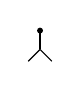
\begin{tikzpicture}[scale=.3]
	\draw (0,0)--(0,.8);
	\draw (0,0)--(.5,-.5);
	\draw (0,0)--(-.5,-.5);
	\draw [fill] (0,.8) circle [radius=0.1];
	\end{tikzpicture}
\end{lrbox}
\newcommand{\unitcoproduct}{% <- this 'right of' is inherited; how to avoid?
	\usebox\preunitcoproduct}

\newsavebox\preleibniz
\begin{lrbox}{\preleibniz}
	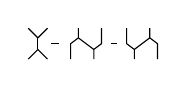
\begin{tikzpicture}[scale=.245]
	\draw (0,.3)--(0,-.3);
	\draw (0,.3)--(.5,.8);
	\draw (0,.3)--(-.5,.8);
	\draw (0,-.3)--(0,.3);
	\draw (0,-.3)--(.5,-.8);
	\draw (0,-.3)--(-.5,-.8);
	
	\draw (.7,0)--(1.1,0);
	\draw (2.1,.8)--(2.1,.3)--(1.7,0)--(1.7,-.8);
	\draw (2.1,.3)--(2.9,-.3);
	\draw (3.3,.8)--(3.3,0)--(2.9,-.3)--(2.9,-.8);
	
	\draw (3.8,0)--(4.1,0);
	\draw (4.6,.8)--(4.6,0)--(5,-.3)--(5,-.8);
	\draw (5,-.3)--(5.8,.3);
	\draw (5.8,.8)--(5.8,.3)--(6.2,0)--(6.2,-.8);	
	\end{tikzpicture}
\end{lrbox}
\newcommand{\leibniz}{% <- this 'right of' is inherited; how to avoid?
	\usebox\preleibniz}

\newsavebox\prebialgebra
\begin{lrbox}{\prebialgebra}
	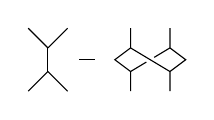
\begin{tikzpicture}[scale=.5]
	\draw (0,.3)--(0,-.3);
	\draw (0,.3)--(.5,.8);
	\draw (0,.3)--(-.5,.8);
	\draw (0,-.3)--(0,.3);
	\draw (0,-.3)--(.5,-.8);
	\draw (0,-.3)--(-.5,-.8);
	
	\draw (.8,0)--(1.2,0);
	
	\draw (2.1,.8)--(2.1,.3)--(1.7,0)--(2.1,-.3)--(2.1,-.8);
	
	\draw (3.1,.8)--(3.1,.3)--(3.5,0)--(3.1,-.3)--(3.1,-.8);

	\draw (2.1,.3)--(3.1,-.3);
	\draw (2.1,-.3)--(2.5,-.06);
	\draw (3.1,.3)--(2.7,.06);	
	\end{tikzpicture}
\end{lrbox}
\newcommand{\bialgebra}{% <- this 'right of' is inherited; how to avoid?
	\usebox\prebialgebra}

\newsavebox\precommutativity
\begin{lrbox}{\precommutativity}
	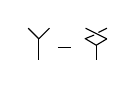
\begin{tikzpicture}[scale=.27]
	\draw (.3,0)--(.3,-1);
	\draw (.3,0)--(.8,.5);
	\draw (.3,0)--(-.2,.5);
	
	\draw (1.2,-.4)--(1.8,-.4);
	
	\draw (3,-.3)--(3,-1);
	\draw (2.5,0)--(3,-.3);
	\draw (3.5,0)--(3,-.3);
	\draw (2.46,0)--(2.9,.18);
	\draw (3.1,.3)--(3.5,.5);
	\draw (3.5,0)--(2.5,.5);
		\end{tikzpicture} 
	\end{lrbox}
	\newcommand{\commutativity}{% <- this 'right of' is inherited; how to avoid?
		\usebox\precommutativity}	

\begin{document}
	\begin{abstract}
	We extend to its ultimate conclusion a line of work started by F. Adams and continued by J.H. Baues, by showing that the classical map comparing the cobar construction on the singular chains of a pointed space and the singular cubical chains on its based loop space preserves an explicitly defined monoidal $E_\infty$-coalgebra structure, which, after M. Mandell, encodes under mild assumptions the homotopy type of the base loop space.
\end{abstract}



%We construct an explicit monoidal $E_\infty$-coalgebra structure on the cobar construction of chains on a reduced simplicial set and, more generally, on the chains of a monoidal cubical set.
%	This involves using a suitable model for the E-infinity operad and a cubical interpretation of the cobar construction.
%Furthermore, we prove that a classical map constructed by F. Adams comparing his cobar construction on the singular chains of a pointed space and the singular cubical chains on its based loop space is a quasi-isomorphism that preserves this structure.
%This work extends to its ultimate conclusion a theorem of H.J. Baues stating that Adams' map preserves a monoidal coalgebra structure.


%
%the singular chains of a pointed space and the singular cubical chains on its based loop space is a quasi-isomorphism that preserves this structure.
%
%
%constructing an explicit monoidal $E_\infty$-coalgebra structure on the cobar construction of chains on a reduced simplicial set, and proving that
%
%
%We construct an explicit monoidal $E_\infty$-coalgebra structure on the cobar construction of chains on a reduced simplicial set and, more generally, on the chains of a monoidal cubical set.
%Furthermore, we prove that a classical map constructed by F. Adams comparing his cobar construction on the singular chains of a pointed space and the singular cubical chains on its based loop space is a quasi-isomorphism that preserves this structure.



%theorem of H.J. Baues stating that Adams' classical monoidal map, comparing his cobar construction on the singular chains of a pointed space and the singular cubical chains on its based loop space, preserves a monoidal coalgebra structure.

% coming from a chain approximation to the diagonal.
%We explicitly construct an $E_\infty$-extension of these monoidal coalgebras making them commutative up to coherent homotopies, and show that Adams' map preserve said structure.
%The importance of $E_\infty$-structures is
%
%It was shown by Mandell that, under mild assumptions, an homotopy commutativity etension of this coalgebra
%We construct an explicit monoidal $E_\infty$-coalgebra structure on the cobar construction of chains on a reduced simplicial set and, more generally, on the chains of a monoidal cubical set, and prove that Adams' map preserves this structure.

	\maketitle
	% !TEX root = ../cobar1.tex

\section{Introduction}

For any topological space $\fX$, its complex of simplicial or cubical singular chains $\Schains(\fX)$ -- regarded as a differential graded (dg) abelian group -- encodes the homology of $\fX$ in its quasi-isomorphism type.
More homotopical information can be stored in the quasi-isomorphism type of this chain complex if considered as a (coassociative) coalgebra, which we will denote $\SchainsA(\fX)$, where the coproduct comes from a natural choice of chain approximation to the diagonal $\fX \to \fX \times \fX$.
For instance, the cohomology ring of $\fX$ is retained, but the action of the Steenrod algebra on its mod~$p$ cohomology is not.

In Mandell's seminal work \cite{mandell2006homotopy_type} it is shown that, when $\fX$ is nilpotent and finite type, the entire homotopy type of $\fX$ can be encoded in the quasi-isomorphism type of this complex if considered as an $E_\infty$-coalgebra, a structure providing $\SchainsA(\fX)$ with coherent homotopies witnessing the derived cocommutativity of the coproduct coming from the strict symmetry of the diagonal map.

The first contribution of this paper is to explicitly endow the cubical singular chains of the based loop space $\loops_x \fX$, with the structure of a monoidal $E_\infty$-coalgebra extending the Serre diagonal.
More specifically, we verify that the monoid structure induced on $\cSchains(\loops_x \fX)$ by the concatenation of loops is compatible with a natural $E_\infty$-coalgebra structure on cubical singular chains, similar to the one defined in \cite{medina2022cube_einfty}.

Applying Adams' cobar construction to the coalgebra of simplicial singular chains of $(\fX, x)$, one obtains another monoidal algebraic model $\cobar \sSchainsA(\fX, x)$ of $\loops_x \fX$ \cite{adams1956cobar}.
More precisely, Adams constructed a natural monoidal chain map $\theta$ from $\cobar \sSchainsA(\fX, x)$ to $\cSchains(\loops_x \fX)$ and proved it to be a quasi-isomorphism if $\fX$ is simply-connected, a statement that also holds true for path-connected spaces after \cite{rivera2018cubical}.
The model $\cobar \sSchainsA(\fX, x)$ is smaller than $\cSchains(\loops_x \fX)$ and unlocks effective analysis of quantitative and qualitative properties of $\loops_x \fX$, as illustrated for instance in \cite{chainalgebraloops} and \cite{adamscobarequivalence}.

The second main contribution of this paper is to make Adams model into a monoidal $E_\infty$-coalgebra and to prove that
\[
\theta \colon \cobar \sSchainsA(\fX, x) \to \cSchains(\loops_x \fX)
\]
respects this higher structure.
Although not pursued in the present article, we remark that the explicit nature of our $E_\infty$-extension invites the study of primary and secondary operations for loops spaces using Adams' model and the tools developed in \cite{medina2021may_st}, \cite{medina2020cartan}, \cite{medina2021adem}, and \cite{medina2021comch}.

Our starting point is groundbreaking work by Baues, which imply statements similar to those in this work but in the category of (coassociative) coalgebras.
Baues reinterpreted Adams' algebraic construction at a deeper geometric level \cite{baues1998hopf}, which allowed him to endow $\cobar \sSchainsA(\fX, x)$ with the structure of a monoidal coalgebra, and to show that $\theta$ preserves this structure.
To prove our statement we interpret Adams' construction at an even deeper categorical level.
We interpret Baues' geometric cobar construction, originally defined for $1$-reduced simplicial sets, as a functor
\begin{equation*}
	\ccobar \colon \sSet^0 \to \Mon_{\cSet},
\end{equation*}
from the category of $0$-reduced simplicial sets to that of monoidal cubical sets.
The key difference with Baues' original work is the use of connections to obtain a natural construction before geometric realization.

Additionally, we need a suitable model of the $E_\infty$-operad endowing cubical chains with a natural $E_\infty$-coalgebra extending the Serre diagonal.
For this we take the operad $\UM$ introduced in \cite{medina2020prop1}.
After proving that its coalgebras form a monoidal category, we show that the functor $\cchainsUM \colon \cSet \to \coAlg_\UM$ -- defined in \cite{medina2022cube_einfty} with a different sign convention -- is monoidal.
This allows us to construct the following extension of Adams and Baues' structures.

\begin{theorem*}
	The following diagram commutes up to natural isomorphisms:
	\[
	\begin{tikzcd} [row sep=small]
		& \Mon_{\coAlg_\UM} \arrow[d] \\
		\Mon_{\cSet} \arrow[ru, "\cchainsUM", out=70, in=180, near start] \arrow[r, "\cchainsA"]
		& \Mon_{\coAlg} \arrow[d] \\
		\sSet^0 \arrow[r, "\cobar \schainsA"] \arrow[u, "\ccobar"]
		& \Mon_{\Ch},
	\end{tikzcd}
	\]
	where the unlabeled arrows are forgetful functors.
\end{theorem*}

In the diagram of the above theorem, the arrow from $\sSet^0$ to $\Mon_{\Ch}$ is Adams' cobar construction, the one from $\sSet^0$ to $\Mon_{\coAlg}$ is Baues' enhancement, and the one from $\sSet^0$ to $\Mon_{\coAlg_{\UM}}$ is our lift.
Additionally, we prove the following statement about Adams's map.

\begin{theorem*}
	For any pointed space $(\fX, x)$,
	\[
	\theta \colon \cobar \sSchainsA(\fX, x) \to \cSchains(\loops_x \fX)
	\]
	is a quasi-isomorphism of monoidal $\UM$-coalgebras.
\end{theorem*}

The fact that $\theta$ respects the monoid structure in $\Ch$ was proven by Adams, whereas the compatibility of the monoid structure with the Serre coalgebra structure was established by Baues.
Our contribution is the compatibility of the monoid structure with a full $E_\infty$-coalgebra extension of Serre's coalgebra.
We also remark that, whereas both Adams and Baues worked in the setting where the underlying space is simply connected, the above theorem does not require any connectivity or finiteness hypotheses.

\subsection*{Related work}

Kadeishvili \cite{kadeishvili1999coproducts, kadeishvili2003cupi} explicitly described monoidal cup-$i$ coproducts on $\cobar \schainsA(X)$ extending Baues coalgebra.
Kadeishvili, as Baues, used cubical methods to define these coproducts and to compare them, in the $1$-connected setting, to cup-$i$ coproducts extending the Serre coalgebra structure on the cubical singular chains of the based loop space.
Additionally, there are several papers \cite{smirnov1990iterated, smith1994cobar, smith2000operads, kadeishvili1998iterating} that predict the existence of, but do not construct, an $E_\infty$-structure on the cobar construction on the chains of simply connected simplicial sets.

On the dual side, Fresse \cite{fresse2003hopf} provided the bar construction of an algebra over the surjection operad with the structure of a comonoid in the category of algebras over the Barratt--Eccles operad.
Additionally, in \cite{fresse2010bar} he used a model category structure on reduced operads \cite{berger2003modelcategory, hinich1997homologicalalgebra} to iterate the bar construction on algebras over cofibrant $E_\infty$-operads.

The use of coalgebras instead of algebras allows us to relate the cobar construction to the based loop space directly --via the Adams map-- without imposing restrictions on the underlying homotopy type, as done by Fresse.
Furthermore, by grounding our approach on the cubical perspective at the heart of Adams' and Baues' seminal papers, we are able to preserve the natural monoidal structures when defining our $E_\infty$-enhancements.
	
\subsection*{Acknowledgements}

We would like to thank Clemens Berger, Matthias Franz, Kathryn Hess, Ralph Kaufmann, Emilio Minichello, Viet-Cuong Pham, Dennis Sullivan, and Mahmoud Zeinalian, for insightful discussions related to this project.

Both authors are grateful for the excellent working conditions of the \textit{Max Planck Institute for Mathematics} in Bonn, Germany.
	% !TEX root = ../cobar1.tex

\section{Conventions and preliminaries}\label{s:preliminaries}

\subsection{Presheaves}

Given categories $\sB$ and $\sC$ with $\sB$ small we denote their associated \textit{functor category} by $\Fun(\sB, \sC)$.
A category is said to be \textit{cocomplete} if any functor to it from a small category has a colimit.
If $\sA$ is small and $\sC$ cocomplete, then the (left) \textit{Kan extension} of $g$ along $f$ exists for any pair of functors $f$ and $g$ in the diagram below, and it is the initial object in $\Fun(\sB, \sC)$ making
\begin{equation*}
	\begin{tikzcd}[column sep=normal, row sep=normal]
		\sA \arrow[d, "f"'] \arrow[r, "g"] & \sC \\
		\sB \arrow[dashed, ur, bend right] & \quad
	\end{tikzcd}
\end{equation*}
commute.
A Kan extension along the \textit{Yoneda embedding}, i.e., the functor
\[
\yoneda \colon \sA \to \Fun(\sA^\op, \Set)
\]
induced by the assignment
\[
a \mapsto \big( a^\prime \mapsto \sA(a^\prime, a) \big),
\]
is referred to as a \textit{Yoneda extension}.
Objects in the image of the Yoneda embedding are said to be \textit{representable}.
Any presheaf $P$ is isomorphic to a colimit of representables presheaves $P \, \cong \colim_{\yoneda(a) \downarrow P} \yoneda(a)$.

\subsection{Chain complexes}

Throughout this article $\k$ denotes a commutative and unital ring and we work over its associated closed symmetric monoidal category of differential (homologically) graded $\k$-modules $(\Ch, \ot, \k)$.
We refer to the objects and morphisms of this category as \textit{chain complexes} and \textit{chain maps} respectively.
We denote by $\Hom(C, C^\prime)$ the chain complex of $\k$-linear maps between chain complexes $C$ and $C^\prime$, and refer to the functor $\Hom(-, \k)$ as \textit{linear duality}.
The $i^\th$ \textit{suspension} functor $s^i \colon \Ch \to \Ch$ is defined at the level of graded modules by $(s^{i}M)_n = M_{n-i}$.


\subsection{Monoids}

A \textit{monoid} $(M, \mu, \eta)$ in a monoidal category $(\sC, \ot, \mathbb{1})$ is an object $M$ together with two morphisms $\mu \colon M \ot M \to M$ and $\eta \colon \mathbb{1} \to M$, called \textit{multiplication} and \textit{unit} respectively, satisfying the usual associativity and unital relations.
We denote the category of monoids in $\sC$ by $\Mon_{\sC}$ and remark that a monoidal functor $\sC \to \sC^\prime$ induces a functor between their categories of monoids $\Mon_\sC \to \Mon_{\sC^\prime}$.

For example, a monoid in $(\Ch, \ot, \k)$ is a differential graded $\k$-algebra. A morphism $f: A \to A'$ in $\Mon_\Ch$ inducing an isomorphism on homology will be called a \textit{monoidal quasi-isomorphism.}

\subsection{Coalgebras}\label{ss:coalgebras}

A \textit{coalgebra} consists of a chain complex $C$ and chain maps $\Delta \colon C \to C \ot C$ and $\varepsilon \colon C \to \k$ satisfying the usual coassociativity and counitality relations.
This notion is equivalent to that of a comonoid in $\Ch$.
Denote by $\coAlg$ the category of coalgebras with morphisms being structure preserving chain maps.
The category $\coAlg$ is symmetric monoidal, with braiding induced from $\Ch$ and structure maps of a product $C \ot C^\prime$ given by
\begin{gather*}
	C \ot C^\prime \xra{\Delta \ot \Delta^\prime}
	(C \ot C) \ot (C^\prime \ot C^\prime) \xra{(23)}
	(C \ot C^\prime) \ot (C \ot C^\prime), \\
	C \ot C^\prime \xra{\varepsilon \ot \varepsilon^\prime}
	\k \ot \k \xra{\cong} \k.
\end{gather*}

A \textit{coaugmentation} on a coalgebra $C$ is a coalgebra map $\nu \colon \k \to C$.
A coalgebra is said to be \textit{coaugmented} if it is equipped with a coaugmentation.
We denote by $\coAlg^\ast$ the category of coaugmented coalgebras with morphisms being coaugmentation preserving coalgebra maps.
A coaugmented coalgebra is a \textit{connected coalgebra} if it is $0$ in negative degrees and the coaugmentation induces an isomorphism $\k \cong C_0$ of $\k$-modules.
We denote by $\coAlg^0$ the full subcategory of $\coAlg^\ast$ defined by these.

\subsection{Simplicial theory}\label{ss:simplicial}

The \textit{simplex category} is denoted by $\simplex$ and its objects by $[n]$.
The category of \textit{simplicial sets} $\Fun(\simplex^\op, \Set)$ is denoted by $\sSet$ and the \textit{standard $n$-simplex} $\yoneda [n] = \simplex(-, [n])$ by $\simplex^n$.
For any simplicial set $X$ we write, as usual, $X_n$ instead of $X[n]$, and identify the elements of $\simplex^n_m$ with increasing tuples $[v_0, \dots, v_m]$ where $v_i \in \{0, \dots, n\}$.

If $X$ is such that $X_0$ is a singleton set we say that $X$ is \textit{reduced}.
We denote the full subcategory of reduced simplicial sets by $\sSet^0$.

We denote the topological $n$-simplex by $\gsimplex^{n}$ and consider the usual adjunction pair defined by the \textit{geometric realization} and \textit{singular complex}
\[
\begin{tikzcd}
	\bars{\ } \colon \sSet  \arrow[r, shift left=.5ex] &
	\Top :\! \sSing. \arrow[l, shift left=.5ex]
\end{tikzcd}
\]

The functor of (normalized) \textit{simplicial chains} $\schains \colon \sSet \to \Ch$ is obtained from the geometric realization and the functor of cellular chains.
When no confusion arises from doing so we write $\chains$ instead of $\schains$ and refer to it simply as the functor of \textit{chains}.
We will denote the functor of (simplicial) \textit{singular chains} $\schains \circ \sSing \colon \Top \to \Ch$ by $\sSchains$.

We modify this construction for a pointed topological space $(\fX,x)$ by only considering maps $\gsimplex^n \to \fX$ sending all vertices to $x$.
This produces a reduced simplicial set $\sSing(\fX,x)$ whose normalized chains we denote by $\sSchains(\fX,x)$.

There is a classical lift of the functor of chains to coalgebras:
\[
\begin{tikzcd}
	& \coAlg \arrow[d] \\
	\sSet \arrow[r, "\schains"] \arrow[ur, "\schainsA", out=70, in=180] & \Ch
\end{tikzcd}
\]
defined, via a Yoneda extension, by the following structure on the chains of standard simplices.
For any $n \in \N$, define $\epsilon \colon \chains(\simplex^n) \to \k$ by
\[
\epsilon \big( [v_0, \dots, v_q] \big) = \begin{cases} 1 & \text{ if } q = 0, \\ 0 & \text{ if } q>0, \end{cases}
\]
and $\Delta \colon \chains(\simplex^n) \to \chains(\simplex^n)^{\ot2}$ by
\[
\Delta \big( [v_0, \dots, v_q] \big) = \sum_{i=0}^q \ [v_0, \dots, v_i] \ot [v_i, \dots, v_q].
\]
We refer to this lift as the \textit{Alexander--Whitney coalgebra} structure on simplicial chains.

If $X$ is a reduced simplicial set then $\schainsA(X)$ becomes a connected coalgebra with the coaugmentation $\nu \colon \k \to \schains(X)$ induced by sending $1$ to the basis element represented by the unique $0$-simplex of $X$.
Hence, the functor $\schainsA$ restricts to a functor
\[
\schainsA \colon \sSet^0 \to \coAlg^0.
\]

\subsection{Cubical theory}\label{ss:cubical}

The objects of the \textit{cube category} $\cube$ are the sets $2^n = \{0, 1\}^n$ with $2^0 = \{0\}$ for $n \in \N$, and its morphisms are generated by the \textit{coface, codegeneracy} and \textit{coconnection} maps defined by
\begin{align*}
	\delta_i^\varepsilon & =
	\mathrm{id}_{2^{i-1}} \times \delta^\varepsilon \times \mathrm{id}_{2^{n-1-i}} \colon 2^{n-1} \to 2^n, \\
	\sigma_i & =
	\mathrm{id}_{2^{i-1}} \times \, \sigma \times \mathrm{id}_{2^{n-i}} \quad \colon 2^{n} \to 2^{n-1}, \\
	\gamma_i & =
	\mathrm{id}_{2^{i-1}} \times \, \gamma \times \mathrm{id}_{2^{n-i}} \quad \colon 2^{n+1} \to 2^{n},
\end{align*}
where $\varepsilon \in \{0,1\}$ and
\[
\begin{tikzcd}
	1 \arrow[r, out=45, in=135, "\delta^0"] \arrow[r, out=-45, in=-135, "\delta^1"'] & 2 \arrow[l, "\sigma"'] &[-10pt] \arrow[l, "\gamma"'] 2 \times 2
\end{tikzcd}
\]
are defined by
\begin{gather*}
	\delta^0(0) = 0, \qquad
	\delta^1(0) = 1, \qquad
	\sigma(0) = \sigma(1) = 0, \qquad \\
	\gamma^1(0,0) = 0, \qquad
	\gamma^1(0,1) = 1, \qquad
	\gamma^1(1,0) = 1, \qquad
	\gamma^1(1,1) = 1.
\end{gather*}
We remark that the cube category without connections will not be considered in this work.

The category of \textit{cubical sets} $\Fun(\cube^\op, \Set)$ is denoted by $\cSet$ and
the \textit{standard $n$-cube} $\yoneda 2^n = \cube(-, 2^n)$ by $\cube^n$.
For any cubical set $Y$ we write, as usual, $Y_n$ instead of $Y(2^n)$.

We denote the topological $n$-cube by $\gcube^{n}$ and consider the usual adjunction pair defined by the \textit{geometric realization} and \textit{singular complex}
\[
\begin{tikzcd}
	\bars{\ } \colon \cSet  \arrow[r, shift left=.5ex] &
	\Top :\! \cSing. \arrow[l, shift left=.5ex]
\end{tikzcd}
\]

The functor of (normalized) \textit{cubical chains} $\cchains \colon \cSet \to \Ch$ is obtained from the geometric realization and the functor of cellular chains.
When no confusion arises from doing so we write $\chains$ instead of $\cchains$ and refer to it simply as the functor of \textit{chains}.
We remark that $\chains(\cube^n)$ is canonically isomorphic to $\chains(\cube^1)^{\ot n}$ and that $\chains(\cube^1)$ is canonically isomorphic to the cellular chains on the topological interval with its usual CW structure.
We use these isomorphisms to denote the elements of $\chains(\cube^n)$ as integral linear combinations monoids of the form $x_1 \ot\dotsb\ot x_n$ with $x_i \in \big\{[0], [0,1], [1] \big\}$.
We will denote the functor of (cubical) \textit{singular chains} $\cchains \circ \cSing \colon \Top \to \Ch$ by $\cSchains$.

There is a classical lift of the functor of cubical chains to the category of coalgebras
\[
\begin{tikzcd}
	& \coAlg \arrow[d] \\
	\cSet \arrow[r, "\cchains"] \arrow[ur, "\cchainsA", out=70, in=180] & \Ch
\end{tikzcd}
\]
defined, using a Yoneda extension, by the tensor product structure (\cref{ss:coalgebras}) defined on $\chains(\cube^n) \cong \chains(\cube^1)^{\ot n}$ via the identification of $\chains(\cube^1)$ and $\chains(\simplex^1)$.
We refer to this lift as the \textit{Serre coalgebra} structure on cubical chains.
We will prove in \cref{ss:cube_einfty revisited} a generalization of the following reformulation of this definition.
\begin{proposition}\label{p:serre coalgebra}
	The functor $\cchainsA \colon \cSet \to \coAlg$ is the unique monoidal functor defined by the coalgebra structure on $\chains(\cube^1)$.
\end{proposition}

%\subsubsection{Cubical chains}
%
%For non-negative integers $m$ and $n$, let $\cube_{\deg}(2^m, 2^n)$ be the subset of \textit{degenerate morphisms} in $\cube(2^m, 2^n)$, i.e., those of the form $\sigma_i \circ \tau$ or $\gamma_i \circ \tau$ with $\tau$ any morphism in $\cube(2^m, 2^{n+1})$.
%The functor of (cubical) \textit{chains} $\cchains \colon \cSet \to \Ch$ is the Yoneda extension of the functor $\cube \to \Ch$ defined next.
%It assigns to an object $2^n$ the chain complex having in degree $m$ the module
%\[
%\frac{\k\{\cube(2^m, 2^n)\}}{\k\{\cube_{\deg}(2^m, 2^n)\}}
%\]
%and differential induced by
%\[
%\partial (\id_{2^n}) = \sum_{i=1}^{n} \ (-1)^i \
%\big(\delta_i^1 - \delta_i^0 \big).
%\]
%To a morphism $\tau \colon 2^n \to 2^{n^\prime}$ it assigns the chain map
%\[
%\begin{tikzcd}[row sep=-3pt, column sep=normal,
%	/tikz/column 1/.append style={anchor=base east},
%	/tikz/column 2/.append style={anchor=base west}]
%	\cchains(\cube^n)_m \arrow[r] & \cchains(\cube^{n^\prime})_m \\
%	\big( 2^m \to 2^n \big) \arrow[r, mapsto] & \big( 2^m \to 2^n \stackrel{\tau}{\to} 2^{n^\prime} \big).
%\end{tikzcd}
%\]
%
%When no confusion arises we write $\chains$ instead of $\cchains$.


%\subsubsection{Cubical singular complex}
%
%Consider the topological $n$-cube
%\[
%\gcube^{n} = \{(x_1, \dots, x_n) \mid x_i \in [0,1]\}.
%\]
%The assignment $2^n \to \gcube^n$ defines a functor $\cube \to \Top$ whose Yoneda extension is known as \textit{geometric realization}.
%It has a right adjoint $\cSing \colon \Top \to \cSet$ given by
%\[
%Z \to \Big(2^n \mapsto \Top(\gcube^n, Z)\Big)
%\]
%and referred to as the \textit{cubical singular complex} of the topological space $Z$.
%We will refer to $\chains(\cSing Z)$ as the \textit{cubical singular chains} of $Z$ and for simplicity denote it by $\cSchains(Z)$.

%\subsubsection{Serre coalgebra}\label{ss:serre coalgebra}
%
%We review a classical lift of the functor of cubical chains to the category of coalgebras
%\[
%\begin{tikzcd}
%	& \coAlg \arrow[d] \\
%	\cSet \arrow[r, "\cchains"] \arrow[ur, "\cchainsA", out=70, in=180] & \Ch.
%\end{tikzcd}
%\]
%Using a Yoneda extension, it suffices to equip the chains on standard cubes with a natural coalgebra structure.
%For any $n \in \N$, define $\epsilon \colon \chains(\cube^n) \to \k$ by
%\[
%\epsilon \left( x_1 \ot \dots \ot x_d \right) = \epsilon(x_1) \dotsm \epsilon(x_n),
%\]
%where
%\[
%\epsilon([0]) = \epsilon([1]) = 1, \qquad \epsilon([0, 1]) = 0,
%\]
%and $\Delta \colon \chains(\cube^n) \to \chains(\cube^n)^{\ot 2}$ by
%\[
%\Delta (x_1 \ot \dots \ot x_n) =
%\sum \pm \left( x_1^{(1)} \ot \dots \ot x_n^{(1)} \right) \ot
%\left( x_1^{(2)} \ot \dots \ot x_n^{(2)} \right),
%\]
%where the sign is determined using the Koszul convention, and we are using Sweedler's notation
%\[
%\Delta(x_i) = \sum x_i^{(1)} \ot x_i^{(2)}
%\]
%for the chain map $\Delta \colon \chains(\cube^1) \to \chains(\cube^1)^{\ot 2}$ defined by
%\[
%\Delta([0]) = [0] \ot [0], \quad \Delta([1]) = [1] \ot [1], \quad \Delta([0,1]) = [0] \ot [0,1] + [0,1] \ot [1].
%\]
%
%Using the canonical isomorphism $\chains(\cube^n) \cong \chains(\cube^1)^{\ot n}$, the coproduct $\Delta$ can be described as the composition
%\[
%\begin{tikzcd}
%	\chains(\cube^1)^{\ot n} \arrow[r, "\Delta^{\ot n}"] & \left( \chains(\cube^1)^{\ot 2} \right)^{\ot n} \arrow[r, "sh"] & \left( \chains(\cube^1)^{\ot n} \right)^{\ot 2},
%\end{tikzcd}
%\]
%where $sh$ is the shuffle map that places tensor factors in odd position first.
	% !TEX root = ../cobar.tex

\section{Operads, props and \pdfEinfty-structures} \label{s:operads and props}

In this section we start by reviewing the basics of the theory of operads and props.
For a more complete presentation we refer the reader to, for example, \cite{markl2008props}.
We then recall from \cite{medina2020prop1} the definition of the finitely presented prop $\M$ having the property that $\UM$ is an $E_{\infty}$-operad.
From the same reference we recall a combinatorial $\UM$-coalgebra structure on simplicial chains and, from \cite{medina2021cubical}, one on cubical chains.

\subsection{Symmetric modules and bimodules}

Let $\S$ be the category whose objects are the natural numbers and whose set of morphisms between $m$ and $n$ is empty if $m \neq n$ and is otherwise the symmetric group $\S_n$.
A (left) \textit{$\S$-module} (resp. $\S$-\textit{bimodule}) is a functor from $\S$ (resp. $\S \times \S^\op$) to $\Ch$.
We respectively denote by $\Smod$ and $\Sbimod$ the categories of left $\S$-modules and of $\S$-bimodules with morphisms given by natural transformations.
The group homomorphisms $\S_n \to \S_n \times \S_1$ induce a forgetful functor $\forget \colon \Sbimod \to \Smod$.
Explicitly, $\forget(\cP)(r) = \cP(1, r)$ for $r \in \N$.
The similarly defined forgetful functor to right $\S$-modules will not be used.

\subsection{Composition structures}

We can define \textit{operads} and \textit{props} by enriching $\S$-modules and $\S$-bimodules with certain composition structures.
For a complete presentation of these concepts we refer to Definition~11 and 54 of \cite{markl2008props}.
Intuitively, using examples defined in the next subsection, operads and props can be understood by abstracting the composition structure naturally present in the left $\S$-module $\End^C$, naturally an operad, and the $\S$-bimodule $\End^C_C$, naturally a prop.
We remark that the prop structure on $\cP$ restricts to an operad structure on $\forget(\cP)$.

\subsection{Representations}

Given a chain complex $C$ define
\[
\End^C(r) = \Hom(C, C^{\otimes r})
\quad \text{and} \quad
\End^C_C(s, r) = \Hom(C^{\otimes s}, C^{\otimes r})
\]
with their natural operad and prop structures respectively.

Given an operad $\cO$, an $\cO$-\textit{structure} on $C$ is an operad morphism $\cO \to \End^C$.
If $C$ is equipped with an $\cO$-\textit{structure} we say it is an $\cO$-\textit{coalgebra}, denoting the category of these by $\coAlg_\cO$.
Similarly for a prop $\cP$, we define the notions of $\cP$-\textit{structure} and of $\cP$-\textit{bialgebra}, denoting their category by $\biAlg_\cP$.

We remark that among these two categories only $\coAlg_\cO$ is cocomplete in general.

\subsection{\pdfEinfty-operads}

Recall that a \textit{free $\S_r$-resolution} of a chain complex $C$ is a quasi-isomorphism $R \to C$ from a chain complex of free $\k[\S_r]$-modules.

An $\S$-module $M$ is said to be $E_{\infty}$ if there exists a morphism of $\S$-modules $M \to \underline{\k}$ inducing for each $r \in \N$ a free $\S_r$-resolution $M(r) \to \k$.
For example, we can obtain one such $\S$-module by using the functor of singular chains and the set, parameterized by $r \in \N$, of maps to the terminal space from models of the universal bundle $\mathrm{E} \S_r$.

An operad is said to be $E_{\infty}$ if its underlying $\S$-module is $E_\infty$.

\subsection{Free constructions} \label{ss:free constructions}

The \textit{free prop} $\free(M)$ generated by an $\S$-bimodule $M$ is constructed using isomorphism classes of directed graphs with no directed loops that are enriched with the following labeling structure.
We think of each directed edge as built from two compatibly directed half-edges.
For each vertex $v$ of a directed graph $\Gamma$, we have the sets $in(v)$ and $out(v)$ of half-edges that are respectively incoming to and outgoing from $v$.
Half-edges that do not belong to $in(v)$ or $out(v)$ for any $v$ are divided into the disjoint sets $in(\Gamma)$ and $out(\Gamma)$ of incoming and outgoing external half-edges.
For any positive integer $n$ let $\overline{n} = \{1, \dots, n\}$ and set $\overline{0} = \emptyset$.
For any finite set $S$, denote the cardinality of $S$ by $|S|$.
The labeling is given by bijections
\[
\overline{|in(\Gamma)|}\to in(\Gamma), \qquad
\overline{|out(\Gamma)|}\to out(\Gamma),
\]
and
\[
\overline{|in(v)|}\to in(v), \qquad
\overline{|out(v)|}\to out(v),
\]
for every vertex $v$.
We refer to the isomorphism classes of such labeled directed graphs with no directed loops as $(n,m)$\textit{-graphs} denoting the set of these by $\graphs(m,n)$.
We use graphs immersed in the plane to represent elements in $\graphs(m,n)$, please see \cref{f:immersion}.
We consider the right action of $\S_n$ and the left action of $\S_m$ on a $(n,m)$-graph given respectively by permuting the labels of $in(\Gamma)$ and $out(\Gamma)$.
This action defines the $\S$-bimodule structure on the free prop
\begin{equation} \label{e:free prop}
	\free(M)(m,n) \ = \bigoplus_{\Gamma \in \graphs(m,n)} \bigotimes_{v \in Vert(\Gamma)} out(v) \otimes_{\S_q} M(p, q) \otimes_{\S_p} in(v),
\end{equation}
where we simplified the notation writing $p$ and $q$ for $\overline{|in(v)|}$ and $\overline{|out(v)|}$ respectively.
The composition structure is defined by (relabeled) grafting and disjoint union.

The \textit{free operad} generated by an $\S$-module is defined analogously using $(1,n)$-graphs only.

\begin{figure}
	\begin{tikzpicture}[scale=.6]
\draw (1,3.7) to (1,3); 

\draw (1,3) to [out=205, in=90] (0,0);

\draw [shorten >= 0cm] (.6,2.73) to [out=-100, in=90] (2,0);

\draw [shorten >= .15cm] (1,3) to [out=-25, in=30, distance=1.1cm] (1,1.5);
\draw [shorten <= .1cm] (1,1.5) to [out=210, in=20] (0,1);

\node at (1,3.9){};
\node at (0,-.32){};
\node at (2,-.32){};

\node at (3,1.5){$\sim$\ \ \ };
\end{tikzpicture}
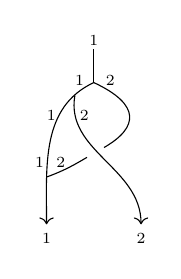
\begin{tikzpicture}[scale=.6]
\draw (1,3.7) to (1,3); 

\draw [->](1,3) to [out=205, in=90] (0,0);

\draw [shorten >= 0cm,->] (.6,2.73) to [out=-100, in=90] (2,0);

\draw [shorten >= .15cm] (1,3) to [out=-25, in=30, distance=1.1cm] (1,1.5);
\draw [shorten <= .1cm] (1,1.5) to [out=210, in=20] (0,1);


\def\x{.8}

\node[scale=\x] at (1,3.9){$\scriptstyle 1$};

\node[scale=\x] at (.7,3.05){$\scriptstyle 1$};
\node[scale=\x] at (1.35,3.05){$\scriptstyle 2$};

\node[scale=\x] at (.1,2.3){$\scriptstyle 1$};
\node[scale=\x] at (.8,2.3){$\scriptstyle 2$};

\node[scale=\x] at (-.15,1.3){$\scriptstyle 1$};
\node[scale=\x] at (.3,1.3){$\scriptstyle 2$};

\node[scale=\x] at (0,-.3){$\scriptstyle 1$};
\node[scale=\x] at (2,-.3){$\scriptstyle 2$};
\end{tikzpicture}
	\caption{Immersed graphs represent labeled directed graphs with the direction implicitly given from top to bottom and the labeling from left to right.}
	\label{f:immersion}
\end{figure}

\subsection{Coalgebras revisited}

We recall the definition of the operad $\As$ controlling coalgebras in the sense of \cref{ss:coalgebras}.
More precisely, $\As$ is defined so that there is a natural isomorphism between $\coAlg_\As$ and $\coAlg$.

\begin{definition}
	Let $\As$ be the operad generated by
	\[
	\counit\,, \qquad \coproduct\,,
	\]
	both in homological degrees $0$ and boundaries
	\[
	\partial\ \counit = 0,
	\hspace*{.6cm}
	\partial\, \coproduct = 0,
	\]
	modulo the operad ideal generated by the relations
	\[
	\leftcounitality\,, \hspace*{.6cm} \rightcounitality\,, \hspace*{.5cm} \coassociativity\,.
	\]
\end{definition}

We remark that this operad is in any arity $r$ isomorphic to the chain complex $\k[\S_r]$ concentrated in degree~$0$.

\subsection{The prop $\M$} \label{ss:definition of M}

We review from \cite{medina2020prop1} the finitely presented $E_{\infty}$-prop $\M$ which, given its small number of generators and relations, is well suited to define $E_{\infty}$-structures.

\begin{definition}
	Let $\M$ be the prop generated by
	\begin{equation} \label{e:generators of M}
		\counit\,, \hspace*{.6cm} \coproduct\,, \hspace*{.6cm} \product,
	\end{equation}
	in degrees $0$, $0$ and $1$ respectively, and boundaries
	\begin{equation} \label{e:boundary of M}
		\partial\ \counit = 0,
		\hspace*{.6cm}
		\partial\, \coproduct = 0,
		\hspace*{.6cm}
		\partial \product = \ \boundary\,,
	\end{equation}
	modulo the prop ideal generated by
	\begin{equation} \label{e:relations of M}
		\leftcounitality\,, \hspace*{.6cm} \rightcounitality\,, \hspace*{.5cm} \coassociativity\,, \hspace*{.6cm} \productcounit.
	\end{equation}
\end{definition}

Explicitly, any element in $\M(m,n)$ can be written as a linear combination of the $(m,n)$-graphs generated by those in \eqref{e:generators of M} via grafting, disjoint union and relabeling, modulo the prop ideal generated by the relations in \eqref{e:relations of M}.
Its boundary is determined, using \eqref{e:free prop}, by \eqref{e:boundary of M}.

Originally this prop was defined without imposing the relation \coassociativity \,.
This is advantageous since in that case the associated reduced operad is a cofibrant resolution of the terminal operad.
Since in this work we are interested in extending the Alexander--Whitney and Serre coalgebras, which are coassociative, we find it convenient to impose this relation, so obtaining an inclusion $\As \to \UM$ and a forgetful functor $\coAlg_\UM \to \coAlg$.

The same proof given in \cite[Theorem 3.3]{medina2020prop1} establishes the following.

\begin{proposition}
	The operad $\UM$ is $E_{\infty}$.
\end{proposition}

We remark that, as proven in \cite{medina2021prop2}, this prop is obtained from applying the functor of cellular chains to a finitely presented prop over the category of CW-complexes.

\subsection{Simplicial \pdfEinfty-structure} \label{ss:e-infty on simplicial}

We review from \cite{medina2020prop1} a natural $\mathcal M$-structure on the chains of standard simplices.
These define, for any simplicial set, a natural $\UM$-structure on its chains generalizing the $E_{\infty}$-coalgebra structures constructed by McClure--Smith \cite{mcclure2003multivariable} and Berger--Fresse \cite{berger2004combinatorial}.

An $\M$-structure is specified by three linear maps, the images of the generators
\[
\counit, \quad \coproduct, \quad \product,
\]
satisfying the relations in the presentation of $\mathcal M$.
For the chains on standard simplices, the first two generators are send respectively to the counit and coproduct of the Alexander--Whitney coalgebra as defined in \cref{ss:aw coalgebra}, and the third generator to an algebraic version of the join $\ast \colon \chains(\simplex^n)^{\otimes 2} \to \chains(\simplex^n)$ defined by
\[
\left[v_0, \dots, v_p \right] \ast \left[v_{p+1}, \dots, v_q\right] = \begin{cases} (-1)^{p+|\pi|} \left[ v_{\pi(0)}, \dots, v_{\pi(q)} \right] & \text{ if } v_i \neq v_j \text{ for } i \neq j, \\
	0 & \text{ otherwise}, \end{cases}
\]
where $\pi$ is the permutation that orders the totally ordered set of vertices, and $(-1)^{|\pi|}$ its sign.

The same proof given in \cite[Theorem 4.2]{medina2020prop1} establishes the following.

\begin{proposition} \label{p:simplicial chain bialgebra}
	For every $n \in \mathbb{N}$, the assignment
	\[
	\counit \mapsto \epsilon, \quad \coproduct \mapsto \Delta, \quad \product \mapsto \ast,
	\]
	defines a natural $\mathcal M$-structure on $\chains(\simplex^n)$ extending the Alexander--Whitney coalgebra.
\end{proposition}

The chains on general simplicial sets are not equipped with an $\M$-structure, but the forgetful functor from $\biAlg_{\M}$ to the cocomplete category $\coAlg_\UM$ allows us to Yoneda extend the induced natural $\UM$-structures on standard simplices to all simplicial sets.
Specifically, we obtain a lift:
\[
\begin{tikzcd}[column sep=normal, row sep=small]
	& \coAlg_\UM \arrow[d] \\
	& \coAlg \arrow[d] \\
	\sSet \arrow[r, "\schains"]
	\arrow[ur, "\schainsA", out=45, in=180]
	\arrow[uur, "\schainsUM", out=90, in=180]
	& \Ch.
\end{tikzcd}
\]

\subsection{Cubical \pdfEinfty-structure} \label{ss:e-infty on cubical}

We review from \cite{medina2021cubical} a natural $\mathcal M$-structure on the chains of standard cubes leading to a natural $\UM$-structure on the chains of any cubical set.

An $\M$-structure is specified by three linear maps, the images of the generators
\[
\counit, \quad \coproduct, \quad \product,
\]
satisfying the relations in the presentation of $\mathcal M$.
For the chains on standard cubes, the first two generators are send respectively to the counit and coproduct of the Serre coalgebra as defined in \cref{ss:serre coalgebra}, and the third generator to a degree one map $\ast \colon \schains(\simplex^n)^{\otimes 2} \to \schains(\simplex^n)$ defined by
\begin{align*}
	(x_1 \otimes \dots \otimes x_n) \ast (y_1 \otimes \dots \otimes y_n) =
	(-1)^{|x|} \sum_{i=1}^n x_{<i} \, \epsilon(y_{<i}) \otimes x_i \ast y_i \otimes \epsilon(x_{>i}) \, y_{>i},
\end{align*}
where
\begin{align*}
	x_{<i} & = x_1 \otimes \dots \otimes x_{i-1}, &
	y_{<i} & = y_1 \otimes \dots \otimes y_{i-1}, \\
	x_{>i} & = x_{i+1} \otimes \dots \otimes x_n, &
	y_{>i} & = y_{i+1} \otimes \dots \otimes y_n,
\end{align*}
with the convention
\[
x_{<1} = y_{<1} = x_{>n} = y_{>n} = 1 \in \k,
\]
and the only non-zero values of $x_i \ast y_i$ are
\[
\ast([0] \otimes [1]) = [0, 1], \qquad \ast([1] \otimes [0]) = -[0, 1].
\]

The same proof given in \cite{medina2020prop1} establishes the following.

\begin{proposition}
	For every $n \in \mathbb{N}$, the assignment
	\[
	\counit \mapsto \epsilon, \quad \coproduct \mapsto \Delta, \quad \product \mapsto \ast,
	\]
	defines a natural $\mathcal M$-structure on $\chains(\cube^n)$ extending the Serre coalgebra.
\end{proposition}

Yoneda extending the induced natural $\UM$-structures on standard simplices to all simplicial sets defines a lift of the functor of cubical chains to $\UM$-coalgebras:
\begin{equation} \label{e:lift of cubical chains to UM-coalgs}
	\begin{tikzcd}[column sep=normal, row sep=small]
		& \coAlg_\UM \arrow[d] \\
		& \coAlg \arrow[d] \\
		\cSet \arrow[r, "\cchains"]
		\arrow[ur, "\cchainsA", out=45, in=180]
		\arrow[uur, "\cchainsUM", out=90, in=180]
		& \Ch.
	\end{tikzcd}
\end{equation}
In the next section we will show that $\cchainsUM$ is a monoidal functor.
	
\section{Monoidal properties of \texorpdfstring{$\UM$}{UM}-coalgebras} \label{s:monoidal}

The first goal of this section is to construct a monoidal structure on $\coAlg_\UM$.
We will do so by providing $\M$ with the structure of a Hopf prop.
Then, we will show that the functor $\cchainsUM \colon \cSet \to \coAlg_{\UM}$ defined in \cref{ss:e-infty on cubical} is monoidal.

\subsection{Monoidal structures on presheaves} \label{ss:day convolution}

Let $\sA$ be a category in $\Cat$ and consider two presheaves $P$ and $P^\prime$ over $\sA$.
Their \textit{Cartesian product} is defined by
\[
(P \times P^\prime)(a) = P(a) \times P^\prime(a),
\]
and, if $(\sA, \otimes)$ is a monoidal category, their \textit{Day convolution product} by
\[
P \otimes P^\prime \, = \! \colim_{\substack{\yoneda(a) \to F \\ \yoneda(a^\prime) \to F^\prime}} \yoneda(a \otimes a^\prime).
\]
These induce natural monoidal structures on the category of presheaves over $\sA$.

In this work we endow $\sSet$ and $\cSet$ with the Cartesian product and Day convolution monoidal structures respectively.


\subsection{Triangulation and its right adjoint} \label{ss:triangulation and its adjoint}

As we recall below, simplicial and cubical sets can be related using the simplicial cubes $(\simplex^1)^{\times n}$.

The \textit{triangulation} functor $\mathcal{T} \colon \cSet \to \sSet$ is defined by
\[
\mathcal{T}(Y) = \colim_{\cube^n \to Y} (\simplex^1)^{\times n}.
\]
It has a right adjoint $\mathcal{U} \colon \sSet \to \cSet$ which is given by the formula
\[
\mathcal{U}(X)_n = \sSet \big( (\simplex^1)^{\times n}, X \big).
\]

With the monoidal structure defined in \cref{ss:day convolution}, the triangulation functor is monoidal.
Thus, it induces a functor
\[
\mathcal{T} \colon \Mon_{\cSet} \to \Mon_{\sSet}
\]
between the associated categories of monoids.

\subsection{Serre coalgebra} \label{ss:serre coalgebra sym monoidal}

Recall that both $\Ch$ and $\coAlg$ are symmetric monoidal categories.
If $\cSet$ is equipped with the Day convolution monoidal structure (\cref{ss:day convolution}), then the functors $\cchains$ and its lift $\cchainsAs$ are symmetric monoidal.
Together with straightforward computations, these statements follow from the fact that the chain complexes $\chains(\cube^p) \otimes \chains(\cube^q)$ and $\chains(\cube^{p+q})$ are canonically isomorphic for any $p, q \geq 0$.

For later reference we record the following consequence of the previous claims and the fact that, for any coalgebra, the braiding $x \otimes y \mapsto (-1)^{\bars{x} \bars{y}} y \otimes x$ is a morphism of coalgebras.

\begin{lemma} \label{l:serre diagonal invariant}
	Let $\sigma \in \S_d$ acting on $\chains(\cube^1)^{\otimes d}$ by permuting tensor factors, then
	\[
	\begin{tikzcd}
	\chains(\cube^1)^{\otimes d} \arrow[r, "\Delta"] \arrow[d, "\sigma"] &
	\chains(\cube^1)^{\otimes d} \otimes \chains(\cube^1)^{\otimes d} \arrow[d, "\sigma \otimes \sigma"] \\
	\chains(\cube^1)^{\otimes d} \arrow[r, "\Delta"] &
	\chains(\cube^1)^{\otimes d} \otimes \chains(\cube^1)^{\otimes d}
	\end{tikzcd}
	\]
	commutes.
\end{lemma}

\subsection{Alexander--Whitney coalgebra}

The functors of simplicial chains $\schains$ and its lift $\schainsAs$ to $\coAlg$ (\cref{ss:aw coalgebra}) are not monoidal in the strict sense.
Nonetheless, with the Eilenberg--Zilber map $\schains(X) \otimes \schains(Y) \to \schains(X \times Y)$ they are lax monoidal functors, a sufficient condition for monoids to be sent to monoids.

\subsection{Hopf operads and \pdfEinfty-bialgebras}

So far we have consider operad and props over the category $\Ch$ but, since $\coAlg$ is also a symmetric monoidal category, we can consider them over $\coAlg$.
That is to say, demand that all defining chain complexes be coalgebras and all compositions be morphisms of these.
We refer to operads and props over $\coAlg$ as \textit{Hopf operads and props} respectively.

If $\cO$ is a Hopf operad, the category $\coAlg_\cO$ is monoidal.
The structure maps of a product of $\cO$-coalgebras $C \otimes C^\prime$ are given by
\[
\begin{tikzcd} [column sep = normal, row sep=large]
\cO(r) \otimes (C \otimes C^\prime) \arrow[r, "\Delta_\cO \otimes \id"] &[10 pt] \cO(r) \otimes \cO(r) \otimes (C \otimes C^\prime) \arrow[d, "Sh"'] & & \\ &
\big(\cO(r) \otimes C \big) \otimes \big( \cO(r) \otimes C \big) \arrow[r] &
C^{\otimes r} \otimes C^{\prime\, \otimes r} \arrow[r, "Sh"] &
(C \otimes C^\prime)^{\otimes r}.
\end{tikzcd}
\]
If $\cO$ is a Hopf $E_\infty$-operad we refer to monoids in $\coAlg_\cO$ as $E_\infty$-\textit{bialgebras}.

Similarly, if $\cP$ is a Hopf prop then its category of representations is also monoidal.

\subsection{Cubical structure on $\M$}

We will now revisit from \cref{ss:definition of M} the definition of $\M$ and provide this prop with a cubical structure.
We will use this in \cref{ss:hopf prop M} to provide $\M$ with the structure of a Hopf prop.

We start with a general observation.
As explained in \cref{ss:free constructions}, the $(m,n)$-part of the free prop generated by an $\S$-module $N$ is given by
\[
\free(N)(m,n) \ = \bigoplus_{\Gamma \in \graphs(m,n)} \bigotimes_{v \in Vert(\Gamma)} out(v) \otimes_{\S_q} N(p, q) \otimes_{\S_p} in(v),
\]
which is well defined only up to a choice of total order on the set of vertices of the $(m,n)$-graphs involved.

In the case we are concern with, the free prop whose quotient defines $\M$ is generated by the $\S$-bimodule $M$ with
\[
M(1,0) = \k \left\{ \; \counit \ \right\}, \qquad
M(1,2) = \k[\S_2] \left\{ \; \coproduct \ \right\}, \qquad
M(2,1) = \k[\S_2^\op] \left\{ \partial_0\! \product \, \right\} \xleftarrow{1 - T} \k[\S_2^\op] \left\{ \, \product \; \right\},
\]
and $M(m,n) = 0$ otherwise.
We notice that the elements $\rightboundary\,$ and $\,\leftboundary\,$ in $\free(M)(2,1)$ are interchanged by the action of $T \in \S_2^\op$.
Let $\widetilde{\M}$ be the quotient of $\free(M)$ by the ideal generated by the identification of $\,\partial_0\! \product$ and $\,\rightboundary\,$, so that the boundary of $\product$ is $\,\boundary\,$.
Consider a basis element of $\widetilde{\M}(m,n)_d$ represented by an immersed $(m,n)$-graph $\Gamma$ with $d$ occurrences of $\product$.
A choice of total order of the vertices of $\Gamma$ defines a chain map
\begin{equation} \label{e:order chain map}
\begin{tikzcd}[row sep=0, column sep=small]
\iota_\Gamma \colon \chains(\cube^d) \arrow[r] & \widetilde{\M}(m,n) \\
\qquad {[0,1]}^{\otimes d} \arrow[r, |->] & \Gamma,
\end{tikzcd}
\end{equation}
referred to as the \textit{characteristic map of $\Gamma$}.
We obtain characteristic maps on $\M$ simply by composing these with the projection $\widetilde{\M} \to \M$ induced from the quotient by the prop ideal generated by the relations \eqref{e:relations of M}.

\subsection{Hopf structure on $\M$} \label{ss:hopf prop M}

We now use the existence of characteristic maps on $\M$ to show it is a prop over $\coAlg$.
We will show the following is well defined in \cref{t:cubical structure on M}.

\begin{definition}
	The \textit{coproduct} $\Delta_\M \colon \M \to \M^{\otimes 2}$ is defined on basis elements $\Gamma$ by
	\[
	\Delta_{\M}(\Gamma) = \iota_\Gamma^{\otimes 2} \circ \Delta \left( [0,1]^{\otimes d} \right),
	\]
	where $d = \bars{\Gamma}$, and the \textit{counit} $\epsilon_\M \colon \M \to \underline{\k}$ by requiring $\epsilon_M(\Gamma) = 1$ if the degree of $\Gamma$ is $0$, where $\underline{\k}$ is the $\S$-bimodule with $\underline{\k}(m, n) = \k$.
\end{definition}

\begin{theorem} \label{t:cubical structure on M}
	The maps $\Delta_\M$ and $\varepsilon_\M$ are well defined and make $\M$ into a Hopf prop.
\end{theorem}

\begin{proof}
	By \cref{l:serre diagonal invariant} these maps are independent of the total order on vertices used to define characteristic maps.

	The linear map $\Delta_\M$ is compatible with the relations defining $\M$ since
	\begin{center}
		\begin{tikzcd}
		\leftcounitcoproduct \arrow[r, "\Delta_\M"] \arrow[d, <->] &[-0pt] \leftcounitcoproduct \otimes \leftcounitcoproduct \arrow[d, <->] \\
		\identity \arrow[r, "\Delta_\M"] & \ \, \identity \otimes \identity \, ,
		\end{tikzcd}
		\quad
		\begin{tikzcd}
		\rightcounitcoproduct \arrow[r, "\Delta_\M"] \arrow[d, <->] &[-0pt] \rightcounitcoproduct \otimes \rightcounitcoproduct \arrow[d, <->] \\
		\identity \arrow[r, "\Delta_\M"] & \ \, \identity \otimes \identity \, ,
		\end{tikzcd}
		\quad
		\begin{tikzcd}
		\leftcomb \arrow[r, "\Delta_\M"] \arrow[d, <->] &[-0pt] \leftcomb \, \otimes \leftcomb \arrow[d, <->] \\
		\rightcomb \arrow[r, "\Delta_\M"] & \, \rightcomb \, \otimes \rightcomb,
		\end{tikzcd}
		\quad
		\begin{tikzcd}
		\productcounit \arrow[r, "\Delta_\M"] \arrow[d, <->] &[-0pt] \counit\ \counit \, \otimes \productcounit + \productcounit \otimes \, \counit\ \counit \arrow[d, <->] \\
		0 \arrow[r, "\Delta_\M"] & \ 0,
		\end{tikzcd}
	\end{center}
	and it is a chain map since
	\begin{center}
		\begin{tikzcd}
		\counit \arrow[r, "\Delta_\M"] \arrow[d, "\partial"'] &[-0pt] \counit \otimes \counit \arrow[d, "\partial"'] \\
		0 \arrow[r, "\Delta_\M"] & \ \, 0 \, ,
		\end{tikzcd}
		\qquad
		\begin{tikzcd}
		\coproduct \arrow[r, "\Delta_\M"] \arrow[d, "\partial"'] &[-0pt] \coproduct \otimes \coproduct \arrow[d, "\partial"'] \\
		0 \arrow[r, "\Delta_\M"] & \ \, 0 \, ,
		\end{tikzcd}
		\qquad
		\begin{tikzcd}
		\product \arrow[r, "\Delta_\M"] \arrow[d, "\partial"'] &[-0pt] \leftboundary \ \otimes \product + \product \otimes\ \rightboundary \arrow[d, "\partial"'] \\
		\rightboundary \,-\, \leftboundary \arrow[r, "\Delta_\M"] &
		\, \rightboundary \otimes \rightboundary \,-\, \leftboundary \otimes \leftboundary\,.
		\end{tikzcd}
	\end{center}
	One can check similarly that $\varepsilon_\M$ is a well defined morphism of $\S$-bimodules.

	Since we are using the Serre coalgebra structure, for each biarity $(m,n)$ we obtain a coalgebra.
	Furthermore, $\Delta_\M$ is compatible with the composition structure since for any pair of characteristic maps $\iota_\Gamma$ and $\iota_{\Gamma^\prime}$, the chain map $\iota_\Gamma \otimes \iota_{\Gamma^\prime}$ is a characteristic map for any composition of $\Gamma$ and $\Gamma^\prime$ with the induce order on vertices.
	The compatibility of $\epsilon_\M$ is immediate.
\end{proof}

\subsection{Monoidal \pdfEinfty-structures}

We now prove the main technical result of this paper.

\begin{lemma} \label{l:cubical e-infty chains are monoidal}
	The functor $\cchainsUM \colon \cSet \to \coAlg_\UM$ is monoidal.
\end{lemma}

\begin{proof}
	It suffices to prove this result for chains on the standard cubes.
	These are equipped with a natural $\M$-structure, and we will prove the stronger statement that the functor $\mathrm{N}^\cube_\M \colon \cube \to \biAlg_{\M}$ is monoidal.

	From \cref{ss:serre coalgebra sym monoidal} we know that the Serre diagonal and the augmentation map are compatible with the monoidal structure on the site $\cube$.
	We need to establish this for the map $\ast$, the image of the generator $\product$.
	Diagrammatically, this is equivalent to the commutativity of
	\begin{equation} \label{e:hopf diagonal and the product}
	\begin{tikzcd}
	\product \otimes \chains(\cube^{p+q})^{\otimes 2} \arrow[d] \arrow[r, "\Delta_\M \otimes Sh"] &[20pt]
	\left(\, \ \leftboundary \ \otimes \product + \product \otimes \ \rightboundary \ \, \right) \otimes \chains(\cube^{p})^{\otimes 2} \otimes \chains(\cube^{q})^{\otimes 2} \arrow[d]\\
	\chains(\cube^{p+q}) \arrow[r, "\cong"] &
	\, \chains(\cube^{p}) \otimes \chains(\cube^{q}).
	\end{tikzcd}
	\end{equation}

	Since this commutativity is immediate for $p = 0$ or $q = 0$ and $\chains(\cube^n) \cong \chains(\cube^1)^{\otimes n}$, we only need to verify it for $p = q = 1$.

	Consider $(x_1 \otimes y_1) \otimes (x_2 \otimes y_2) \in \chains(\cube^1)^{\otimes 2} \otimes \chains(\cube^1)^{\otimes 2}$.
	We have
	\[
	\begin{split}
	\big((\id \otimes \varepsilon) \otimes \ast \ + \ \ast \otimes (\varepsilon \otimes \Delta)\big) \ (-1)^{\bars{y_1} \bars{x_2}} \ (x_1 \otimes x_2) \otimes (y_1 \otimes y_2) \ & = \\
	(-1)^{\bars{y_1} \bars{x_2} + \bars{x_1} + \bars{x_2} + \bars{y_1}} \ x_1 \cdot \varepsilon(x_2) \otimes y_1 \ast y_2 \ & + \
	(-1)^{\bars{y_1} \bars{x_2} + \bars{x_1}} \ x_1 \ast x_2 \otimes \varepsilon(y_1) \ast y_2.
	\end{split}
	\]
	The first summand on the right hand side of this identity is non-zero only if $\bars{x_2} = \bars{y_1} = \bars{y_2} = 0$, whereas the second is non-zero only if $\bars{x_1} = \bars{x_2} = \bars{y_1} = 0$, so the above is also equal to
	\begin{equation} \label{e:join is monoidal 1}
	(-1)^{\bars{x_1}} \ x_1 \cdot \varepsilon(x_2) \otimes y_1 \ast y_2 \ + \
	x_1 \ast x_2 \otimes \varepsilon(y_1) \ast y_2.
	\end{equation}
	On the other hand,
	\begin{align*}
	(x_1 \otimes y_1) \ast (x_2 \otimes y_2) \ & =\
	(-1)^{\bars{x_1} + \bars{y_1}} \ (x_1 \ast x_2) \otimes \varepsilon(y_1) \cdot y_2 \ +\
	(-1)^{\bars{x_1} + \bars{y_1}} \ x_1 \cdot \varepsilon(x_2) \otimes (y_1 \ast y_2) \\ \ & =\
	(x_1 \ast x_2) \otimes \varepsilon(y_1) \cdot y_2 \ +\
	(-1)^{\bars{x_1}} \ x_1 \cdot \varepsilon(x_2) \otimes (y_1 \ast y_2),
	\end{align*}
	which is equal to \eqref{e:join is monoidal 1} as claimed.
\end{proof}

%	In diagrammatic terms,
%	\[
%	\begin{tikzcd}
%	\coproduct \otimes \chains(\cube^{p+q}) \arrow[r, "\Delta_\M \otimes Sh"] \arrow[d] &[20pt]
%	\left( \ \coproduct \otimes \coproduct \ \right) \otimes
%	\chains(\cube^{p}) \otimes \chains(\cube^{q}) \arrow[d] \\
%	\chains(\cube^{p+q})^{\otimes 2} \arrow[r, "Sh"] &
%	\chains(\cube^{p})^{\otimes 2} \otimes \chains(\cube^{q})^{\otimes 2}
%	\end{tikzcd}
%	\]
%	and
%	\[
%	\begin{tikzcd}
%	\counit \ \otimes \chains(\cube^{p+q}) \arrow[r, "\Delta_\M \otimes Sh"] \arrow[d] &[20pt]
%	\left( \ \counit \ \otimes \ \counit \ \right) \otimes
%	\chains(\cube^{p}) \otimes \chains(\cube^{q}) \arrow[d] \\
%	R \arrow[r, "\cong"] &
%	R \otimes R
%	\end{tikzcd}
%	\]
%	commute.

	
\section{Adams's map as an \texorpdfstring{$E_{\infty}$}{E-infty}-bialgebra quasi-isomorphism} \label{s:theorem1}

The goal of this section is to prove \cref{t:1st main thm in the intro}.
Explicitly, we construct a natural $E_{\infty}$-bialgebra structure on $\cobar \schains(X)$ for any reduced simplicial set $X$ (\cref{l:lift of cobar to e-infty}); and show that when $X$ is the singular complex of a topological space $(Z, z)$, Adams' comparison map $\theta_Z \colon \cobar \sS(Z, z) \to S^{\cube}(\loops_z Z)$ is a quasi-isomorphism of $E_\infty$-bialgebras (\cref{l:adams comparison is an e-infty bialgebra map}).

The first goal is achieved using a categorical reformulation of Baues' geometric cobar construction (\cref{ss:cubical cobar}) together with the natural $\UM$-coalgebra structure defined on cubical chains (\cref{ss:e-infty on cubical}) and its monoidal properties (\cref{l:cubical e-infty chains are monoidal}).
The second goal is obtained by factoring Adams' comparison map through this cubical model (\cref{ss:factorization of adams}).

\subsection{Adams' map}\label{adamsmaps}

In \cite{adams1956cobar}, Adams constructed a natural map of algebras
\begin{equation} \label{e:adams map 2}
\theta_Z \colon \cobar \sS(Z, z) \to S^{\cube}(\loops_z Z),
\end{equation}
for any pointed topological space $(Z, z)$.
The construction is based on a collection of continuous maps
\[
\theta_n \colon \gcube^{n-1} \to P(\gsimplex^n;0,n),
\]
where $P(\gsimplex^n;0,n)$ denotes the topological space of Moore paths in $\gsimplex^n$ from the $0$-th vertex $v_0$ to the $n$-th vertex $v_n$.
These maps are constructed inductively so that following equations are satisfied:
\begin{enumerate}
	\item $\theta_1(0)\colon \gcube^1 \to \gsimplex^1$ is the path $\theta_1(0)(s) = sv_1 +(1-s)v_0$.
	\item $\theta_n \circ e_j^0 = P(d_j) \circ \theta_{n-1}$.
	\item $\theta_n \circ e_j^1 = (P(f_j) \circ \theta_j) \cdot (P(l_{n-j}) \circ \theta_{n-j})$.
\end{enumerate}
In the above equations $f_j\colon \gsimplex^j \rightarrow \gsimplex^n$ and $l_{n-j}\colon \gsimplex^{n-j} \rightarrow \gsimplex^n$ denote the first $j$-th face map and last $(n-j)$-th face map of $\gsimplex^n$, respectively, and
$e_j^0,e_j^1\colon \gcube^{n-1} \rightarrow \gcube^{n}$ denote the $j$-th bottom and top cubical face maps, respectively.
For any continuous map of spaces $f \colon Z \to Z'$, we denote by $P(f) \colon P(Z) \to P(Z')$ the induced map at the level of spaces of paths.
Given any two composable paths $\alpha$ and $\beta$, the dot symbol in $\alpha \cdot \beta$ denotes the composition (or concatenation) of paths.

Adams' map $\theta_Z$ is now given as follows.
For any singular $1$-simplex $\sigma \in S^{\Delta}_1(Z, z)$ let
\[
\theta_Z([\sigma]) = P(\sigma) \circ \theta_1 - c_z,
\]
where $c_z \in S^{\cube}_0(\loops_z Z)$ is the singular $0$-cube determined by the constant loop at $z \in Z$.
For any singular $n$-simplex $\sigma \in S^{\Delta}_n(Z, z)$ with $n>1$, let
\[
\theta_Z([\sigma]) = P(\sigma) \circ \theta_n.
\]
Since the underlying graded algebra of $\cobar \sS(Z, z)$ is free, we may extend the above to an algebra map $\theta_Z \colon \cobar \sS(Z, z) \to S^{\cube}(\loops_z Z)$.
The compatibility equations for the maps $\theta_n$ imply that $\theta_Z$ is a chain map.

We will construct an $E_{\infty}$-bialgebra structure on $\cobar \sS(Z, z)$ and show that, when $S^{\cube}(\loops_z Z)$ is equipped with the $E_{\infty}$-coalgebra structure described in \cref{ss:e-infty on cubical}, the map $\theta_Z$ is a map of $E_{\infty}$-coalgebras.
With this goal in mind, we describe a categorical version of Adams' constructions.

\subsection{Necklical sets}

We construct a cubical model for the based loop space using necklical sets, a notion related to both simplicial sets and cubical sets.
Similar constructions and results to those appearing in this and the next three sub-sections may be found in \cite{baues1980geometry}, \cite{berger1995loops}, \cite{baues1998hopf}, \cite{dugger2011rigidification}, \cite{galvez2020hopf}, and \cite{rivera2018cubical, rivera2019path}.

Let us first consider the subcategory $\simplex_{*,*}$ of the simplex category $\simplex$ with the same objects and morphisms given by functors $f \colon [n] \to [m]$ satisfying $f(0) = 0$ and $f(n) = m$.
It is a strict monoidal category when equipped with the monoidal structure $[n] \otimes [m] = [n+m]$, thought of as identifying the elements $n \in [n]$ and $0 \in [m]$, and unit given by $[0]$.
In passing, we mention that this category is $\op$-dual to the augmented simplex category, a form of Joyal duality.

The \textit{necklace category} $\Nec$ is obtained from $\simplex_{*,*}$ as follows.
Thinking of $\simplex_{*,*}$ as a monoid in $\Cat$, we first apply the bar construction to it and produce a simplicial object in $\Mon_{\Cat}$ which, after realization, defines the strict monoidal category $\Nec$.
We denote the monoidal structure by
\[
\vee \colon \Nec \times \Nec \to \Nec.
\]
We describe $(\Nec, \vee)$ in more explicit terms.
The objects of $\Nec$, called \textit{necklaces}, are freely generated by the objects of $\simplex_{*,*}$ through the monoidal structure $\vee$.
Namely, the set of objects of $\Nec$ is given by
\[
\big\{ [n_1] \vee \dots \vee[n_k] \mid n_i, k \in \N_{>0} \big\}
\]
together with $[0]$ serving as the monoidal unit.

The morphism of $\Nec$ are generated through the monoidal structure by the following four types of morphisms:
\begin{enumerate}
	\item $\partial^j \colon [n-1] \to [n]$ for $j = 1, \dots, n-1$
	\item $\Delta_{[j], [n-j]} \colon [j] \vee [n-j] \to [n]$ for $j = 1, \dots, n-1$
	\item $s^j \colon [n+1] \to [n]$ for $j = 0, \dots, n$ and $n>0$, and
	\item $s^0 \colon [1] \to [0]$.
\end{enumerate}
We may identify $\Nec$ with a full sub-category of the category of double pointed simplicial sets $\sSet_{*,*}$ as follows.
Consider the functor
\[
\mathcal{S} \colon \Nec \to \sSet_{*,*}
\]
 induced by sending any necklace $T = [n_1] \vee \dots \vee[n_k]$ to the simplicial set
\[
\mathcal{S}(T) = \simplex^{n_1} \vee \dots \vee \simplex^{n_k},
\]
where the wedge symbol now means we identify the last vertex of $\simplex^{n_i}$ with the first vertex of $\simplex^{n_{i+1}}$ for $i = 1, \dots, k-1$ and the two base points are given by the first vertex of $\simplex^{n_1}$ and the last vertex of $\simplex^{n_k}$.
Then $\mathcal{S}$ is a fully faithful functor, so $\Nec$ may be identified with the full sub-category of $\sSet_{*,*}$ having as objects those double pointed simplicial sets of the form $\simplex^{n_1} \vee \dots \vee \simplex^{n_k}$.
The \textit{dimension} of a necklace $T = [n_1] \vee \dots \vee[n_k]$ is defined by $\dim(T) = n_1 + \dots + n_k-k$.

The category of \textit{necklical sets} is the functor category $\nSet = \Fun[\Nec^{\op}, \Set]$.
The \textit{Yoneda embedding}
\[
\mathcal{Y} \colon \Nec \to \nSet,
\]
is the functor induced by by $T \mapsto \Nec(-,T)$.

The category of necklical sets $\nSet$ is a (non-symmetric) monoidal category when equipped with the Day convolution structure $\otimes \colon \nSet \times \nSet \to \nSet$ (\cref{ss:day convolution}) given by
\[
K \otimes K' \, = \colim_{\substack{\mathcal{Y}(T) \to K, \\ \mathcal{Y}(T')\to K'}} \mathcal{Y}(T \vee T').
\]

\subsection{From necklaces to cubes}

We now describe a categorical version of Adams' maps
\[
\theta_n \colon \gcube^{n-1} \to P(\gsimplex^{n};0,n)
\]
by constructing a monoidal functor
\[
\mathcal{P} \colon \Nec \to \cube.
\]

We first set $\mathcal{P}([0])=2^0$.
On any other necklace $T \in \Nec$ we define $\mathcal{P}( T )= 2^{\dim(T)}$.
In order to define $\mathcal{P}$ on morphisms, it is sufficient to consider the following cases.
\begin{enumerate}
	\item For any $\partial^j \colon [n] \to [n+1]$ such that $0< j<{n+1}$, define $\mathcal{P}(\partial^j) \colon 2^{n-1}\to 2^{n}$ to be the cubical coface functor $\mathcal{P}(f)= \delta_0^{j}$.

	\item For any $\Delta_{[j], [n+1-j]} \colon [j] \vee [n+1-j] \to [n+1]$ such that $0<j<n+1$, define
	\[
	\mathcal{P}(\Delta_{[j], [n+1-j]}) \colon 2^{n-1}\to 2^{n}
	\]
	to be the cubical coface functor $\mathcal{P}(f)=\delta_1^{j}$.

	\item We now consider morphisms of the form $s^j \colon [n+1] \to [n]$ for $n>0$.
	If $j=0$ or $j=n$, then $\mathcal{P}(f) \colon 2^n \to 2^{n-1}$ is defined to be the cubical codegeneracy functor $\mathcal{P}(s^j)= \varepsilon^{j}$.
	If $0<j<n$, then we define $\mathcal{P}(s^j) \colon 2^n \to 2^{n-1}$ to be the cubical coconnection functor $\gamma^{j}$.

	\item For $s^0 \colon [1] \to [0]$ we define $\mathcal{P}(s^0) \colon 2^0 \to 2^0$ to be the identity functor.
\end{enumerate}

\begin{remark}
	The functor $\mathcal{P}$ is neither faithful or full.
	However, for any necklace $T' \in \Nec$ with $\dim(T')=n+1$ and any cubical coface functor $\delta_{\epsilon}^j \colon 2^n \to 2^{n+1}$ for $0 \leq j \leq n+1$, there exists a unique pair $(T, f \colon T \hookrightarrow T')$, where $T \in \Nec$ with $\dim(T)=n$ and $f \colon T \hookrightarrow T'$ is an injective morphism in $\Nec$, such that $\mathcal{P}(f) = \delta_{\epsilon}^j $.
\end{remark}

The functor $\mathcal{P} \colon \Nec \to \cube$ induces an adjunction between $\cSet$ and $\nSet$ with right and left adjoint functors given respectively by
\[
\mathcal{P}^\ast \colon \cSet \to \nSet,
\qquad \text{and} \qquad
\mathcal{P}_{!} \colon \nSet \to \cSet.
\]
Explicitly, for a cubical set $Y \colon \cube^\op \to \Set$,
\[
\mathcal{P}^\ast(Y)= Y \circ \mathcal{P}^\op,
\]
and for a necklical set $K \colon \Nec^\op \to \Set$,
\[
\mathcal{P}_{!}(K) \ =
\colim_{\mathcal{Y}(T) \to K} \mathcal{P}(T) \ \cong
\colim_{\mathcal{Y}(T) \to K} \cube^{\dim(T)}.
\]
Since $\mathcal{P}$ is a monoidal functor, the functor $\mathcal{P}_{!} \colon \nSet \to \cSet$ is a monoidal as well.

\subsection{Cubical cobar construction} \label{ss:cubical cobar}

Using the framework of necklical sets, we may reinterpret a Baues' geometric cobar construction from \cite{baues1998hopf} as a functor
\[
\ncobar \colon \sSet^0 \to \Mon_{\nSet},
\]
which we now define.

For any reduced simplicial set $X$, we define a necklical set $\ncobar(X) \colon \Nec^\op \to \Set$ having as necklical cells all necklaces inside $X$; namely
\[
\ncobar(X) \, = \! \colim_{\mathcal{S}(T) \to X} \mathcal{Y}(T).
\]
The product
\[
\ncobar(X) \otimes \ncobar(X) \to \ncobar(X)
\]
is induced by the monoidal structure $\vee \colon \Nec \times \Nec \to \Nec$ given by concatenation of necklaces.
More precisely, using that
\[
\mathcal{Y}(T) \cong \colim_{(R \to T) \in \Nec \downarrow T} \mathcal{Y}(R),
\]
we may describe the product
\[
\ncobar(X) \otimes \ncobar(X) \to \ncobar(X)
\]
by
\[
[f\colon \mathcal{S}(T) \to X, R \to T] \otimes [f'\colon \mathcal{S}(T') \to X, R' \to T'] \mapsto [f \vee g\colon \mathcal{S}(T\vee T') \to X, R \vee R'\to T \vee T'],
\]
where $(f\colon \mathcal{S}(T) \to X), (f'\colon \mathcal{S}(T') \to X) \in \mathcal{S} \downarrow X$, $ (R\to T) \in \Nec \downarrow T$, and $(R' \to T') \in \Nec \downarrow T'$.
The bracket notation $[f\colon \mathcal{S}(T) \to X, R\to T]$ denotes the equivalence class of a pair $(f \colon \mathcal{S}(T) \to X, R \to T)$ in the colimit defining $\ncobar(X)$.

We may now define the \textit{cubical cobar construction}
\[
\ccobar \colon \sSet^0 \to \Mon_{\cSet}
\]
as the composition
\[
\ccobar = \mathcal{P}_! \, \ncobar.
\]
This reinterpretation of Baues construction in terms of cubical sets was also studied in \cite{rivera2018cubical}.

\subsection{Relation to the cobar construction}

We now relate the cubical cobar functor $\ccobar \colon \sSet^0 \to \Mon_{\cSet}$ to the cobar construction $\cobar \colon \coAlg \to \Mon_{\Ch}$ (\cref{ss:cobar construction}).

\begin{lemma} \label{l:ccobar and cobar}
	There is a natural isomorphisms of functors
	\[
	\cchains \ccobar \cong \cobar \schains \colon \sSet^0 \to \Mon_{\Ch}.
	\]
\end{lemma}

\begin{proof}
	Denote by $\iota_n \in (\cube^n)_n$ the top dimensional non-degenerate element of the standard $n$-cube $\cube^n$.
	Note that for a reduced simplicial set $X$, we may represent any non-degenerate $n$-cube $\alpha \in (\mathcal{P}_!(\ncobar(X)))_n$ as a pair $\alpha = [\sigma \colon \mathcal{Y}(T) \to X, \iota_n]$ for some $T = [n_1] \vee \dots \vee [n_k] \in \Nec$ with $\dim(T) = n_1 + \dots + n_k - k = n$.

	To define an algebra map
	\[
	\varphi_X \colon \cchains(\mathcal{P}_!(\ncobar(X))) \xra{\cong} \cobar \schains(X)
	\]
	it suffices to define it on any generator of the form $\alpha=[\sigma \colon \simplex^{n+1} \to X, \iota_{n}]$, i.e., when $T$ is of the form $T = [n+1]$, for some $n \geq 0$.
	If $n = 0$ let $\varphi_X(\alpha)= [\overline{\sigma}] + 1_\k$, where $[\overline{\sigma}] \in s^{-1} \overline{ \schains(X)} \subset \cobar \schains(X)$ denotes the (length $1$) generator in the cobar construction of $\schains(X)$ determined by $\sigma \in X_{n+1}$ and $1_\k$ denotes the unit of the underlying ring $\k$.
	If $n > 0$, we let $\varphi_X(\alpha)=[\overline{\sigma}]$.
	A straightforward computation yields that this gives rise to a well defined isomorphism of algebras, which is compatible with the differentials, and natural with respect to maps of simplicial sets.
\end{proof}
A similar result to \cref{l:ccobar and cobar} was observed in the case of $1$-reduced simplicial sets in Section 3.5 of \cite{berger1995loops}.

\subsection{An $E_{\infty}$-bialgebra structure on the cobar construction} \label{ss:e-infty on cobar}

The original cobar construction of Adams produces monoids in $\Ch$.
Baues enriched this construction to produce monoids in $\coAlg$.
He did this by using a version of the isomorphism $\cchains \ccobar \cong \cobar \schains$ of \cref{l:ccobar and cobar} and the Serre coalgebra on cubical chains.
Since $\ccobar$ produces monoids in $\cSet$ and $\cchainsAs$ is monoidal, the functor $\cchainsAs \ccobar$ produces bialgebras, as claimed.

After \cite{medina2021cubical}, we know that cubical chains can be enriched with an $E_\infty$-coalgebra structure extending the Serre coalgebra (\cref{ss:e-infty on cubical}).
This $\UM$-structure can be transferred via $\cchains \ccobar \cong \cobar \schains$ to provide the cobar construction with and $E_\infty$-structure extending Baues coalgebra structure.
Furthermore, thanks to \cref{l:cubical e-infty chains are monoidal}, we know that $\cchainsUM$ is monoidal and therefore, $\cchains \ccobar$ produces monoids in $\coAlg_{\UM}$, i.e., $E_\infty$-bialgebras.
This discussion proves the first half of \cref{t:1st main thm in the intro}, which we collect in the following.

\begin{lemma} \label{l:lift of cobar to e-infty}
	The functor $\cchainsUM$ is monoidal and fits in the following diagram commuting up to a natural isomorphism:
	\[
	\begin{tikzcd}
	& \Mon_{\coAlg_\UM} \arrow[d] \\
	\Mon_{\cSet} \arrow[ru, "\cchainsUM", out=70, in=180] \arrow[r, "\cchainsAs"]
	& \Mon_{\coAlg} \arrow[d] \\
	\sSet^0 \arrow[r, "\cobar \schains"] \arrow[u, "\ccobar"]
	& \Mon_{\Ch}.
	\end{tikzcd}
	\]
\end{lemma}

\subsection{Steenrod operations}

Throughout this subsection let us consider $\k$ to be the finite field $\Fp$ and $X$ a reduced simplicial set.

Since, \cref{l:ccobar and cobar}, $\cobar \schains(X)$ is isomorphic to the chains on a cubical set, its mod $p$ homology is a priori equipped with a right action of the Steenrod algebra \cite{steenrod1962cohomology, milnor1958steenrod}.
As an application of the explicit construction of a natural $\UM$-coalgebra structure on $\cobar \schains(X)$, we can describe at the chain level this action using the constructions of \cite{medina2020maysteenrod}.
More explicitly, let $\Cp$ be the cyclic group of order $p$ and
\[
\begin{tikzcd} [column sep = .5cm]
\mathcal W(p) = \Fp[\Cp]\{e_0\} & \arrow[l, "\,T"'] \Fp[\Cp]\{e_1\} & \arrow[l, "\,N"'] \Fp[\Cp]\{e_2\} & \arrow[l, "\,T"'] \dotsb
\end{tikzcd}
\]
be the minimal free resolution of $\Fp$ as an $\Fp[\Cp]$-module.
Consider the $\Cp$-equivariant quasi-isomorphism $\psi_\UM \colon W(p) \to \UM(p)$ constructed in \cite{medina2020maysteenrod}, and denote by $\Psi^{\cobar}$ its composition with the morphism $\UM \to \End^{\cobar \schains(X)}$ defining our $E_\infty$-coalgebra structure on $\cobar \schains(X)$.

For $p = 2$, the Steenrod square $P_s$ is represented by the map sending a representative $\mu$ of a class in the $k\th$ homology of $\cobar \schains(X)$ to the following element in its double linear dual:
\[
\mu \mapsto
\Big( \alpha \mapsto (\alpha \otimes \alpha) \big( \psi^{\cobar}(e_{k+2s})(\mu) \big) \Big).
\]
Similarly, for $p$ an odd prime, we have that the action of the Steenrod operations $\beta^\varepsilon P_{s}$ where $\varepsilon = 0,1$ are represented by
\[
\mu \mapsto
\Big( \alpha \mapsto \alpha^{\otimes p} \big( (-1)^p \, \nu(q) \, \psi^{\cobar}(e_{(2s-q)(p-1)-\varepsilon})(\mu) \big) \Big)
\]
where
\[
q = -k -2s(p-1)+\varepsilon, \qquad
\nu(q) = (-1)^{q(q-1)m/2}(m!)^q, \qquad
m = (p-1)/2.
\]

The map $\psi^{\cobar}$, being a special case of the map $\psi^\cube$ defined in \cite{medina2020maysteenrod}, can be described effectively, and it has been implemented in the specialized computer algebra system \texttt{ComCH} \cite{medina2021computer}.
In similar effective manner, for the mod 2 case, explicit Cartan and Adem coboundaries \cite{medina2020cartan, medina2020adem} can be described for the cochain level Steenrod squares of the cobar construction.

\subsection{Factorization of Adams' map} \label{ss:factorization of adams}

We now use the ideas developed so far to study the based loop space of a pointed topological space $(Z, z)$.

Using the natural isomorphism of algebras
\[
\cobar \schains (\sSing(Z, z)) \cong \cchains \ccobar (\sSing(Z, z))
\]
of \cref{l:ccobar and cobar}.
Adams' map can be factored as
\begin{equation} \label{e:factorization of adams}
\theta_Z \colon \cobar \sS(Z, z) \xrightarrow{\cong}
\cchains \ccobar(\sSing(Z, z)) \xrightarrow{\cchains(\Theta)}
S^{\cube}(\loops_z Z),
\end{equation}
where second map is given by applying the cubical chains functor $\cchains \colon \Mon_{\cSet} \to \Mon_{\Ch}$ to the map of monoidal cubical sets
\[
\Theta \colon \ccobar(\sSing(Z, z)) \to \cSing(\loops_z Z)
\]
determined through the monoid structure by sending an $n$-simplex $(\sigma \colon \gsimplex^n \to Z)$ to the singular $(n-1)$-cube
\[
P(\sigma) \circ \theta_n \colon \gcube^{n-1} \to \loops_z Z,
\]
where the maps $\theta_n \colon \gcube^{n-1} \to P(\gsimplex^n;0,n)$ are those defined by Adams and discussed in \cref{adamsmaps}.


\subsection{Adams's map as an $E_{\infty}$-bialgebra quasi-isomorphism}

Adams' comparison map
\[
\theta_Z \colon \cobar \sS(Z, z) \to S^{\cube}(\loops_z Z)
\]
was originally identified to be a morphism of monoids in $\Ch$ which, if applied to simply-connected spaces, induces a homology isomorphism.
Baues showed that $\theta_Z$ is in fact a morphism of monoids in $\coAlg$, i.e., of bialgebras.
Whereas, using that $\sSing(Z, z)$ is a fibrant reduced simplicial set, the second named author and M. Zeinalian \cite{rivera2018cubical} showed that for a possibly non-simply connected pointed space $(Z,y)$ the algebras $\cobar \sS(Z, z)$ and $S^{\cube}(\loops_zZ)$ are quasi-isomorphic.
Later on, the second named author and S. Saneblidze
\cite{rivera2019path} showed that $\Theta \colon \ccobar(\sSing(Z, z)) \to \cSing(\loops_z Z)$ is a weak homotopy equivalence monoids in $\cSet$.

We now show that $\theta_Z$ is in fact a quasi-isomorphism of $E_{\infty}$-bialgebras.
Considering the factorization \eqref{e:factorization of adams} of Adams' comparison map.
The isomorphism is by construction one of $\UM$-bialgebras, whereas the second map, induced from a weak-equivalence of monoids in $\cSet$, is also a morphism of $\UM$-bialgebras
since $\cchainsUM$ is monoidal (\cref{l:cubical e-infty chains are monoidal}).
We summarize this discussion, which constitutes the second half of \cref{t:1st main thm in the intro}, in the following.

\begin{lemma} \label{l:adams comparison is an e-infty bialgebra map}
	Adams' comparison map $\theta_Z \colon \cobar \sS(Z, z) \to S^{\cube}(\loops_z Z)$ is a quasi-isomorphism of $E_{\infty}$-bialgebras or, more specifically, of monoids in $\coAlg_\UM$ for any pointed space $(Z, z)$.
\end{lemma}

	
\section{Relation to Kan's loop group construction} \label{s:theorem2}

The goal of this section is to prove \cref{t:2nd main thm in the intro}.
Explicitly, we construct an $E_{\infty}$-coalgebra structure on the extended cobar construction of \cite{hess2010cobar} together with a natural zig-zag of quasi-isomorphisms of $E_{\infty}$-coalgebras connecting it to the chains on the Kan loop group.

Our comparison uses the rigidification functor, a construction introduced by Cordier and used by Lurie, Dugger, and Spivak in the theory of $\infty$-categories, as a middle object to relate the Kan loop group and the cubical cobar construction.
The rigidification functor is naturally isomorphic to the triangulation of the cubical cobar construction, as explained in \cref{Candgcobar}.
In \cref{CandG}, we show that a localized version of the rigidification functor agrees, up to homotopy, with the Kan loop group.
\cref{t:2nd main thm in the intro} then follows by applying the corresponding functors of normalized chains and comparing these via the Serre--Cartan map, as explained in the last three subsections.
Our arguments rely on several classical results from homotopy theory, which we review for completeness.

\subsection{Kan's loop group construction}

Recall that simplicial sets form a combinatorial model for the homotopy theory of spaces.
This may be expressed using the language of model categories by stating that the adjoint functors
\[
\bars{\ \cdot\ } \colon \sSet \leftrightarrows \mathsf{Top} :\! \sSing
\]
defines a Quillen equivalence between model category structures, where $\Top$ is equipped with the classical \textit{Quillen model structure} and $\sSet$ with the \textit{Kan-Quillen model structure}.
We refer to the induced model structure on $\sSet^0$ by the same name.

The based loop space of a reduced simplicial set may be modeled in purely combinatorial terms through the \textit{Kan loop group functor}
\[
\kan \colon \sSet^0 \to \sGrp
\]
defined as follows.
For any reduced simplicial set $X$ each $\kan(X)_n$ is the group with one generator $\overline{x}$ for every simplex $x \in X_{n+1}$ modulo the relation $\overline{s_0(x)} = e$, where $e$ denotes the identity element of the group.

The face and degeneracy maps are defined by the following equations:
\[
\delta_0(\overline{x}) = \overline{\delta_1(x)} \cdot (\overline{\delta_0(x)})^{-1}, \qquad \quad
\delta_n(\overline{x}) = \overline{\delta_{n+1}(x)} \text{ for } n>0, \qquad \quad
s_n(\overline{x}) = \overline{s_{n+1}(x)}.
\]

Berger showed that this construction models the based loop space as a topological monoid.
More precisely, he showed that for any reduced simplicial set $X$, the geometric realization of the Kan loop group $\bars{\kan(X)}$ is weak homotopy equivalent, as a topological monoid, to the based loop space $\loops \bars{X}$ on the geometric realization of $X$ \cite{berger1995loops}.

Using Kan's ideas, Quillen constructed a model category structure on the category $\sGrp$ of simplicial groups determined by
weak equivalences and fibrations being maps of simplicial groups whose underlying maps of simplicial sets are weak homotopy equivalences and Kan fibrations, respectively.
We call this model category structure the \textit{Kan model structure} on $\sGrp$.

The Kan loop group functor has a right adjoint $\classifying \colon \sGrp \to \sSet^0$ modeling the classifying space of a simplicial group.
As proven for example in \cite[Chapter V]{goerss2009simplicial} we have the following.

\begin{proposition} \label{p:kan adjuntion}
	The adjunction
	\[
	\kan \colon \sSet^0 \leftrightarrows \sGrp :\! \classifying
	\]
	defines a Quillen equivalence when $\sSet^0$ and $\sGrp$ are equipped respectively with the Kan-Quillen and the Kan model category structures.
\end{proposition}

\subsection{Extended cobar construction}

The proof that Adams' map in \cref{t:1st main thm in the intro} is a quasi-isomorphism relies on the fibrancy of the singular complex.
In general, for an arbitrary reduced simplicial set $X$, the cobar construction $\cobar \schains(X)$ is not quasi-isomorphic to $S^{\cube}(\loops|X|)$, the singular cubical chains on the based loop space of the geometric realization of $X$.
This is true, however, if $X$ is $1$-connected.

In \cite{hess2010cobar}, it is described how to formally invert the elements of $X_1$ inside $\cobar \schains(X)$ to obtain the correct quasi-isomorphism type.
The resulting model, called the \textit{extended cobar construction}, is then compared, as an algebra, to the chains on the Kan loop group construction $\kan(X)$.
We now review these constructions and, in \cref{ss:extended cubical cobar}, reinterpret them in categorical terms.

Denote the composition of the functor of chains and the cobar construction by
\[
\A \defeq \cobar \schains \colon \sSet^0 \to \Mon_{\Ch},
\]
and define the functor
\[
\Ahat \colon \sSet^0 \to \Mon_{\Ch}
\]
to be the localization of the set of $0$-cycles
\[
A_X = \{ [\overline{\sigma}]+1_\k \mid \sigma \in X_1 \} \subset \A(X)_0
\]
in the associative algebra $\A(X)$.

The algebra $\Ahat(X)$ coincides with Hess--Tonk's extended cobar construction applied to the coalgebra $\schains(X)$ at the $\k$-basis of the degree $1$-elements given by the set $X_1$.
More precisely, using the notation of \cite{hess2010cobar}, we have $\Ahat(X) = \widehat{\cobar} \schains(X)$, where the fixed basis in the latter is given the set $X_1$.
Note that the extended cobar construction is not a functorial construction with respect to maps in $\coAlg$ since it depends on a choice of basis of the degree one $\k$-module in the underlying coalgebra.
It is, however, functorial with respect to maps of reduced simplicial sets and that is how we have interpreted it.

Furthermore, for any reduced simplicial set $X$, the natural quasi-isomorphism of algebras
\[
\phi_X \colon \Ahat(X) \to \schains(\kan(X))
\]
constructed in \cite{hess2010cobar} induces a natural isomorphism
\[
H_0(\Ahat(X)) \cong \k[\pi_1(X)].
\]

\subsection{Extended cubical cobar construction} \label{ss:extended cubical cobar}

We now want to lift the localization procedure used to define $\Ahat$ to the level of monoidal cubical sets.

We define a functor
\[
\ncobarE \colon \sSet^0 \to \Mon_{\nSet}
\]
by formally adding inverses for every $0$-dimensional necklace $\sigma \colon \simplex^1 \to X$ in $\ncobar(X)$ subject to the usual relations together with the higher degenerate necklaces generated by these new formal elements.

Define the \textit{extended cubical cobar construction}
\[
\ccobarE \colon \sSet^0 \to \Mon_{\cSet}
\]
to be the composition of functors $\ccobarE = \mathcal{P}_{!} \ncobarE$.

As an immediate consequence of \cref{l:ccobar and cobar}, we obtain the following isomorphism after localizing.

\begin{corollary}
	There is a natural isomorphism of functors
	\[
	\cchains \ccobarE \, \cong \Ahat \colon \sSet^0 \to \Mon_{\Ch}.
	\]
\end{corollary}

\begin{proof}
	The isomorphism $\varphi_X \colon \cchains(\ccobar(X))\to \A(X)$
	of \cref{l:ccobar and cobar} induces a bijection between the sets
	$X_1$ and $A_X$.
	Hence, the result follows directly from the definitions of $\ccobarE(X)$ and $\Ahat(X)$, where the sets $X_1$ and $A_X$, respectively, have been formally inverted.
\end{proof}

\subsection{The functor $\Ahat_{\UM}$} \label{s:ahatum}

Define the functor
\[
\Ahat_{\coAlg} \colon \sSet^0 \to \Mon_{\coAlg}
\]
as the composition
\[
\Ahat_{\coAlg} = \cchainsAs \ccobarE.
\]
Similarly define
\[
\Ahat_{\UM} \colon \sSet^0 \to \Mon_{\coAlg_{\UM}}
\]
as the composition
\[
\Ahat_{\UM} = \cchainsUM \ccobarE.
\]

It follows directly from the definitions that $\Ahat_{\coAlg}$ is a lift of $\Ahat$, and $\Ahat_{\UM}$ is a lift $\Ahat_{\coAlg}$.
This discussion constitutes the first half of \cref{t:2nd main thm in the intro}, which we collect in the following.

\begin{lemma}
The functor $\Ahat_\UM \colon \sSet^0 \to \Mon_{\coAlg_\UM}$ fits into a commutative diagram
	\[
	\begin{tikzcd}[row sep=small]
	& \Mon_{\coAlg_\UM} \arrow[d] \\
	& \Mon_{\coAlg} \arrow[d] \\
	\sSet^0
	\arrow[r, "\Ahat"', ]
	\arrow[ru, "\Ahat_{\coAlg}"', out=45, in=180]
	\arrow[ruu, "\Ahat_\UM", out=90, in=180]
	& \Mon_{\Ch}.
	\end{tikzcd}
	\]
\end{lemma}

\subsection{Rigidification and homotopy coherent nerve}

In order to relate the functors $\ccobarE \colon \sSet^0 \to \Mon_{\cSet}$ and $\kan \colon \sSet^0\to \sGrp$ we introduce a third construction, the \textit{rigidification functor}
\[
\rigid \colon \sSet^0 \to \Mon_{\sSet},
\]
which is obtained by restricting to $\sSet^0$ a more general construction
\[
\rigid \colon \sSet \to \Cat_{\simplex},
\]
where $\Cat_{\simplex}$ denotes the category of small categories enriched over $\sSet$.
We now recall the construction and refer to \cite{dugger2011rigidification} for further details.

Given integers $0 \leq i \leq j$ denote by $P_{i,j}$ the category whose objects are all the subsets of $\{i, i+1, \dots, j\}$ containing both $i$ and $j$ and morphisms are inclusions.
For each integer $n \geq 0$ define $\rigid(\simplex^n) \in \Cat_{\simplex}$ to have the set $\{0, \dots, n\}$ as objects and if $i \leq j$, define $\rigid(\simplex^n)(i,j)= N(P_{i,j})$, where $N$ is the ordinary nerve functor.
If $j < i$, $\rigid(\simplex^n)(i,j) = \emptyset$.
The composition law in $\rigid(\simplex^n)$ is induced by the functor $P_{j,k} \times P_{i,k} \to P_{i,k}$ defined as the union of sets.
The assignment $[n] \mapsto \rigid(\simplex^n)$ defines a cosimplicial object in $\Cat_{\simplex}$.
For any reduced simplicial set $S$ we can now define
\[
\rigid(S) = \colim_{\simplex^n \to S} \rigid(\simplex^n).
\]

The functor $\rigid$ has a right adjoint, called the \textit{homotopy coherent nerve functor} and denoted by
\[
\nerve \colon \Cat_{\simplex} \to \sSet,
\]
whose $n$-simplices are given by
\[
\nerve(\mathcal{C})_n = \Hom_{\Cat_{\simplex}}(\rigid(\simplex^n), \mathcal{C}).
\]

The category of simplicial sets also serves as a combinatorial framework to model the homotopy theory of $\infty$-categories.
More precisely, both Joyal and Lurie independently described a model category structure on $\sSet$ whose weak equivalences are given by a sub-collection of the weak homotopy equivalences called the \textit{categorical equivalences}, cofibrations are injective maps, and fibrant objects are quasi-categories.
This model category is known as the \textit{Joyal model structure}.
The Kan-Quillen model structure is a left Bousfield localization of the Joyal model structure obtained by localizing the single morphism $\simplex^1 \to \simplex^0$.

On the other hand, Bergner constructed a model structure on $\Cat_{\simplex}$ having as weak equivalences those maps of simplicially enriched categories that induce a weak homotopy equivalence between the simplicial sets of morphisms and are essentially surjective after passing to the homotopy categories.
Fibrant objects are categories enriched over Kan complexes.
This model category is known as the \textit{Bergner model structure}.

The adjunction between rigidification and the homotopy coherent nerve yields an equivalence of homotopy theories modeling the $\infty$-categories.
More precisely, we have the following statement, which is one of the main results of \cite{dugger2011mappingspaces}.

\begin{proposition} \label{joyalbergner}
	The adjunction
	\[
	\rigid \colon \sSet \leftrightarrows \Cat_{\simplex} :\!\nerve
	\]
	induces a Quillen equivalence when $\sSet$ is equipped with the Joyal model structure and $\Cat_{\simplex}$ with the Bergner model structure.
\end{proposition}

The next result, which is an observation of the second named author and Zeinalian, relates the cubical cobar construction and the rigidification functor via the triangulation functor as defined in \cref{ss:triangulation and its adjoint}.

\begin{proposition} \label{Candgcobar}
	The composition
	\[
	\mathcal{T} \, \ccobar \colon \sSet^0 \to \Mon_{\sSet}
	\]
	is naturally isomorphic to
	\[
	\rigid \colon \sSet^0 \to \Mon_{\sSet}.
	\]
\end{proposition}

The above statement is Proposition 5.3 in \cite{rivera2018cubical}, where $\ccobarE$ is denoted by $\rigid_{\cube_c}$.
The proof relies on a description of the rigidification functor in terms of necklaces due to Dugger and Spivak \cite{dugger2011rigidification}.
\cref{Candgcobar} also holds in the many-object setting, but we do not need this level of generality for the purposes of this article.

\subsection{The rigidification functor and Kan's loop group construction}

Denote by
\[
\iota \colon \sGrp \to \Mon_{\sSet}
\]
the natural fully faithful embedding through which we may regard simplicial groups as simplicial monoids. The starting point of the comparison between the rigidification functor and Kan's loop group functor is the following statement about their adjoints, which is Proposition 2.6.2 in \cite{hinich2007deformation}.

\begin{proposition} \label{p:hinich}
	For any simplicial group $\mathcal{G} \in \sGrp$, we have a natural weak homotopy equivalence
	\[
	\psi_{\mathcal{G}} \colon \classifying(\mathcal{G}) \xrightarrow{\simeq} \nerve\iota(\mathcal{G}).
	\]
\end{proposition}

We now relate the rigidification functor $\rigid$ and the Kan loop group functor $G$.
First we introduce some notation.
The embedding $\iota \colon \sGrp \to \Mon_{\sSet}$ has a left adjoint, which we denote by
\[
\mathcal{L} \colon \Mon_{\sSet} \to \sGrp.
\]
More precisely, this is the functor from simplicial monoids to simplicial groups given by formally inverting all morphisms (degree by degree) subject to the usual relations.
If $M \in \Mon_{\sSet}$ and $A \subseteq M_0$ is a subset of $0$-morphisms, we denote by $\mathcal{L}_AM$ the simplicial monoid obtained by formally inverting the elements of $A$, i.e. the pushout
\[
\mathcal{L}_AM= M \coprod_A \mathcal{L}F(A),
\]
where $F(A)$ is the monoid freely generated by the set $A$ regarded as a discrete simplicial monoid.

\begin{lemma} \label{CandG}
	There are natural weak equivalences of simplicial monoids
	\[
	\localization_{X_1} \! \rigid(X) \xra{\simeq} \localization \rigid(X) \xra{\simeq} \kan(X)
	\]
	for any reduced simplicial set $X$.
\end{lemma}

\begin{proof}
	Since $\rigid$ is a left Quillen functor and every simplicial set $X$ is cofibrant in the Joyal model structure, it follows from \cref{joyalbergner} that the simplicially enriched category $\rigid(X)$ is a cofibrant.
	Hence, Proposition 9.5 of \cite{dwyer1980simplicial} implies that the natural inclusion $\localization_{X_1} \! \rigid(X) \to \localization \rigid(X)$ is a weak equivalence of simplicially enriched categories.

	By \cref{p:hinich} we have that $\psi_{\kan(X)} \colon \classifying \kan(X) \xrightarrow{\simeq} \nerve \iota(\kan(X))$ is a weak homotopy equivalence for any reduced simplicial set $X$.
	By \cref{p:kan adjuntion}, we have a weak homotopy equivalence $X \xrightarrow{\simeq} \classifying \kan(X)$ given by the unit of the adjunction.
	Composing these two maps we obtain a weak homotopy equivalence
	\[
	X \xrightarrow{\simeq} \nerve\iota(\kan(X)).
	\]
	The Quillen equivalence of \cref{joyalbergner} localizes to a Quillen equivalence
	\[
	\localization \rigid \colon \sSet^0 \leftrightarrows \sGrp \colon \nerve \iota
	\]
	when $\sSet^0$ is equipped with the Kan-Quillen model structure and $\sGrp$ with the model structure of \cref{p:kan adjuntion}.
	It follows that the adjoint of the weak homotopy equivalence $X \xra{\simeq} \nerve \iota(\kan(X))$ is a weak equivalence of simplicial groups
	\[
	\localization \rigid(X) \xra{\simeq} \kan(X),
	\]
	which finishes the proof.
\end{proof}


\subsection{Localized cubical cobar and the Kan loop group}

We have the following comparison between the triangulation of the localized geometric cobar construction and the Kan loop group.

\begin{corollary} \label{widehatgcobarandG}
	There is a natural weak equivalence of simplicial monoids
	\[
	\mathcal{T} \ccobarE(X) \xrightarrow{\simeq} \kan(X)
	\]
	for any reduced simplicial set $X$.
\end{corollary}

\begin{proof}
	After localizing the isomorphism of \cref{Candgcobar} at the $1$-simplices, we obtain a natural isomorphism of simplicial monoids
	\[
	\mathcal{T} \ccobarE(X) \cong \localization_{X_1} \! \rigid(X).
	\]
	Hence, the result follows from \cref{CandG}.
\end{proof}

 The above statement should be understood as a lift of Hess and Tonk's quasi-isomorphism between the extended cobar construction and the chains on the Kan loop group to the level of simplicial sets.
In fact, it is explained in \cite{minichello2021path} how the weak equivalence
\[
\mathcal{T} \ccobarE(X) \cong \mathcal{L}_{X_1} \! \rigid(X) \to \kan(X)
\]
obtained in \cref{widehatgcobarandG}
 can be described explicitly in terms of the Szczarba operators used in \cite{hess2010cobar}.
More precisely, Hess and Tonk's comparison map is precisely the composition
\[
\Ahat(X) = \cchains(\ccobarE(X)) \to \schains(\mathcal{T}\ccobarE(X)) \to \schains (\kan(X)),
\]
where the first map is determined by the shuffle quasi-isomorphism
$\cchains(\cube^n)\to \schains \big( (\simplex^1)^{\times n} \big)$ from a cube to its triangulation and the second map is induced by the weak equivalence of \cref{widehatgcobarandG} after applying chains.
The first map in this composition preserves the coassociative coalgebra structures but not the $\UM$-coalgebra structures.
Nevertheless, in the following sections, we describe a zig-zag of quasi-isomorphisms of $E_{\infty}$-coalgebras between $\cchains(\ccobarE(X))$ and $\schains(\mathcal{T}\ccobarE(X))$.

\subsection{Serre--Cartan comparison map}

We review from \cite{medina2021cubical} the relationship between the $E_\infty$-structures defined on simplicial chains in \cref{ss:e-infty on simplicial} and on cubical chains in \cref{ss:e-infty on cubical}.

In \cite[p.442]{serre1951homologie}, the \textit{Serre--Cartan collapse} $\gcube^n \to \gsimplex^n$ was introduced and used to define a natural quasi-isomorphism of coalgebras $\sS(Z) \to \cS(Z)$ for any topological space $Z$.
This map factors as the composition
\[
\schains(\sSing(Z)) \xra{\CS_{\sSing(Z)}}
\cchains(\mathcal{U} \sSing(Z)) \to
\cchains(\cSing(Z)),
\]
where the first map $\CS_X$, referred to as the \textit{Serre--Cartan comparison map}, is a quasi-isomorphism defined for any simplicial set $X$, and the second map is induced from a morphism of cubical sets.

Although both $\schains(X)$ and $\cchains(\mathcal{U} X)$ have natural $\UM$-structures, the map $\CS_X$ is not a morphism of $\UM$-coalgebras for a generic simplicial set $X$.
Nevertheless, after restriction of their $\UM$-structures via an inclusion of $E_\infty$-operads $\USL \to \UM$, the Cartan-Serre comparison map becomes a morphism of $E_\infty$-coalgebras.
The operad $\USL$ is generated as a suboperad of $\UM$ by all immerse connected graphs of the form
\begin{equation*}
\begin{tikzpicture}[scale=1]
\draw (0,0)--(0,-.6) node[below, scale=.75]{$1$};
\draw (0,0)--(.5,.5);
\draw (-.3, .3)-- (-.2,.5) node[scale=.75] at (-.2,.7) {\qquad $1\, \ \ 2\ \ ...\ \ k_1$};
\draw (-.5,.5)--(0,0);
\node[scale=.75] at (.11,.4){$..$.};

\node[scale=.75] at (1,0){$\cdots$};
\node[scale=.75] at (1,-.9){$\cdots$};

\draw (2,0)--(2,-.68) node[scale=.75, below]{$r$};
\draw (2,0)--(2.5,.5);
\draw (1.7, .3)--(1.8,.5) node[scale=.75] at (1.78,.7) {\qquad $1\, \ \ 2\ \ ...\ \ k_r$};
\draw (1.5,.5)--(2,0);
\node[scale=.75] at (2.11,.4){$..$.};

\draw (1,2.5)--(1,3) node[scale=.75, above]{$1$};
\draw (1,2.5)--(0,2) node[scale=.75, below]{$1$};
\draw (.25,2.125)--(.5,2) node[scale=.75, below]{$2$};
\draw (.5,2.25)--(1,2) node[scale=.75, below]{$3$};
\draw (1,2.5)--(2,2) node[scale=.75, below]{\ \quad $n + r$};
\node[scale=.75] at (1.5,1.75){$\cdots$};

\node[scale=.75] at (1,1.3) {$\vdots$};

\node at (2.85,0){};
\end{tikzpicture}
\end{equation*}
where there are no hidden vertices and the strands are joined so that the associated maps $\{1, \dots, k_j\} \to \{1, \dots, n+k\}$ are order-preserving.
From \cite{medina2021cubical} we have the following.

\begin{proposition} \label{p:simplicialandcubical}
	The suboperad $\USL$ of $\UM$ is an $E_\infty$-operad and the Cartan-Serre comparison map
	\[
	\CS_X \colon \schains(X) \to \cchains(\mathcal U X)
	\]
	is a natural quasi-isomorphism of $\USL$-coalgebras for any simplicial set $X$.
\end{proposition}

We will denote by $\chains_\USL$ the functor of (cubical or simplicial) chains lifted to $\coAlg_\USL$.
We remark that the inclusion $\As \to \UM$ factors through $\USL$ so $\chains_\USL$ is also a lift to a category of $E_\infty$-coalgebras of the functors $\chains_\As$ to $\coAlg$.

\subsection{A zig-zag of $E_\infty$-coalgebras}
The $E_{\infty}$-coalgebra structures on the simplicial chains on a triangulated cubical set $Y$ and on the cubical chains on $Y$ are related as follows.

\begin{lemma} \label{l:zigzag}
	For any cubical set $Y$ there are natural quasi-isomorphisms of $\USL$-coalgebras
	\begin{equation} \label{e:zig-zag of quasi-isos}
	\schainsUSL(\mathcal{T}Y) \xra{\simeq}
	\cchainsUSL(\mathcal{U}\mathcal{T}Y) \xleftarrow{\simeq}
	\cchainsUSL(Y).
	\end{equation}
\end{lemma}

\begin{proof}
	The first map in \eqref{e:zig-zag of quasi-isos} is a quasi-isomorphism of $\USL$-coalgebras by \cref{p:simplicialandcubical}.
	Whereas the second is induced by the morphism of cubical sets $Y \to \mathcal{U} \mathcal{T} (Y)$ given by the unit of the adjunction
	\[
	\mathcal{T} \colon \cSet \leftrightarrows \sSet :\! \mathcal{U}
	\]
	of \cref{ss:triangulation and its adjoint}.
	The unit map is in fact a weak homotopy equivalence of cubical sets since the adjunction defines a Quillen equivalence between the Kan-Quillen model structure and an analogue model structure on $\cSet$ in which all objects are cofibrant \cite{cisinski2006presheaves}.
	Hence, the unit map induces a quasi-isomorphism of $\USL$-coalgebras after applying the cubical chains functor.
\end{proof}

\subsection{The extended cobar construction and the chains on the Kan loop group}

Applying \cref{l:zigzag} to $Y = \ccobarE(X)$, we obtain that $\schainsUSL (\mathcal{T} \ccobarE(X))$ and $\cchainsUSL(\ccobarE(X)) = \Ahat_{\USL}(X)$ are quasi-isomorphic via a zig-zag of natural maps of $\USL$-coalgebras.
By \cref{widehatgcobarandG} we have a weak equivalence of simplicial monoids
\[
\mathcal{T}\ccobarE(X) \xrightarrow{\simeq} \kan(X)
\]
for any reduced simplicial set $X$.
By naturality, we have an induced quasi-isomorphism of $\USL$-coalgebras
\[
\schainsUSL \big( \mathcal{T} \ccobarE(X) \big) \xra{\simeq}
\schainsUSL (\kan(X)).
\]
Therefore, $\Ahat_{\USL}(X)$ and $\schainsUSL(\kan(X))$ are quasi-isomorphic through a zig-zag of natural maps of $\USL$-coalgebras, as desired.
We summarize this discussion in the following lemma, constituting the second half of \cref{t:2nd main thm in the intro}.

\begin{lemma}
	For any reduced simplicial set $X$, there is a zig-zag of natural quasi-isomorphisms of $\USL$-coalgebras between $\Ahat_\USL(X)$ and $\schainsUSL(\kan(X))$.
\end{lemma}
	\sloppy
    \printbibliography
\end{document}
